%% Author: PGL  Porta Mana
%% Created: 2015-11-04T09:20:08+0100
%% Last-Updated: 2017-05-15T22:57:55+0200
%%%%%%%%%%%%%%%%%%%%%%%%%%%%%%%%%%%%%%%%%%%%%%%%%%%%%%%%%%%%%%%%%%%%%%
%Report-no: ***
\documentclass{article}

% if you need to pass options to natbib, use, e.g.:
% \PassOptionsToPackage{numbers, compress}{natbib}
% before loading nips_2017
%
% to avoid loading the natbib package, add option nonatbib:
% \usepackage[nonatbib]{nips_2017}

\usepackage[final,nonatbib]{nips_2017}
\newcommand*{\firstdraft}{4 November 2015}
\newcommand*{\pdftitle}{Hidden  assumptions on population size\\in the maximum-entropy method}
\newcommand*{\headtitle}{\pdftitle}
\newcommand*{\pdfauthor}{P.G.L.  Porta Mana, V. Rostami, E. Torre}

\usepackage{newtxmath}
%\usepackage{pifont}
%\usepackage{fontawesome}
\usepackage[T1]{fontenc} 
\input{glyphtounicode} \pdfgentounicode=1
\usepackage[utf8]{inputenx}
\usepackage{newunicodechar}
% \newunicodechar{Ĕ}{\u{E}}
% \newunicodechar{ĕ}{\u{e}}
% \newunicodechar{Ĭ}{\u{I}}
% \newunicodechar{ĭ}{\u{\i}}
% \newunicodechar{Ŏ}{\u{O}}
% \newunicodechar{ŏ}{\u{o}}
% \newunicodechar{Ŭ}{\u{U}}
% \newunicodechar{ŭ}{\u{u}}
% \newunicodechar{Ā}{\=A}
% \newunicodechar{ā}{\=a}
% \newunicodechar{Ē}{\=E}
% \newunicodechar{ē}{\=e}
% \newunicodechar{Ī}{\=I}
% \newunicodechar{ī}{\={\i}}
% \newunicodechar{Ō}{\=O}
% \newunicodechar{ō}{\=o}
% \newunicodechar{Ū}{\=U}
% \newunicodechar{ū}{\=u}
% \newunicodechar{Ȳ}{\=Y}
% \newunicodechar{ȳ}{\=y}

\newcommand*{\bmmax}{3} % reduce number of bold fonts, before bm
\newcommand*{\hmmax}{0} % reduce number of heavy fonts, before bm
\usepackage{textcomp}
\usepackage{amsmath}
\usepackage{mathtools}
\setlength{\multlinegap}{0pt}

\usepackage{amssymb}
\usepackage{amsxtra}

\usepackage[british]{babel}\selectlanguage{british}
\newcommand*{\langfrench}{\foreignlanguage{french}}
\newcommand*{\langgerman}{\foreignlanguage{german}}
\newcommand*{\langitalian}{\foreignlanguage{italian}}
\newcommand*{\langswedish}{\foreignlanguage{swedish}}
\newcommand*{\langlatin}{\foreignlanguage{latin}}
\newcommand*{\langnohyph}{\foreignlanguage{nohyphenation}}

\usepackage[autostyle=false,autopunct=false,english=british]{csquotes}
\setquotestyle{american}

\let\openbox\relax
\usepackage{amsthm}
\newcommand*{\QED}{\textsc{q.e.d.}}
\renewcommand*{\qedsymbol}{\QED}
\theoremstyle{remark}
\newtheorem{note}{Note}
\newtheorem*{remark}{Note}
\newtheoremstyle{innote}{\parsep}{\parsep}{\footnotesize}{}{}{}{0pt}{}
\theoremstyle{innote}
\newtheorem*{innote}{}

\usepackage{bm}

\iffalse
\usepackage[shortlabels,inline]{enumitem}
\SetEnumitemKey{para}{itemindent=\parindent,leftmargin=0pt,listparindent=\parindent,parsep=0pt,itemsep=\topsep}
% \begin{asparaenum} = \begin{enumerate}[para]
% \begin{inparaenum} = \begin{enumerate*}
\setlist[enumerate,2]{label=\alph*.}
\setlist[enumerate]{leftmargin=\parindent}
\setlist[itemize]{leftmargin=\parindent}
\setlist[description]{leftmargin=\parindent}
\fi

%% With euler font cursive for Greek letters - the [1] means 100% scaling
\DeclareFontFamily{U}{egreek}{\skewchar\font'177}%
\DeclareFontShape{U}{egreek}{m}{n}{<-6>s*[0.95]eurm5 <6-8>s*[0.95]eurm7 <8->s*[0.95]eurm10}{}%
\DeclareFontShape{U}{egreek}{m}{it}{<->s*[0.95]eurmo10}{}%
\DeclareFontShape{U}{egreek}{b}{n}{<-6>s*[0.95]eurb5 <6-8>s*[0.95]eurb7 <8->s*[0.95]eurb10}{}%
\DeclareFontShape{U}{egreek}{b}{it}{<->s*[0.95]eurbo10}{}%
\DeclareSymbolFont{egreeki}{U}{egreek}{m}{it}%
\SetSymbolFont{egreeki}{bold}{U}{egreek}{b}{it}% from the amsfonts package
\DeclareSymbolFont{egreekr}{U}{egreek}{m}{n}%
\SetSymbolFont{egreekr}{bold}{U}{egreek}{b}{n}% from the amsfonts package
% Take also \sum, \prod, \coprod symbols from Euler fonts
\DeclareFontFamily{U}{egreekx}{\skewchar\font'177}
\DeclareFontShape{U}{egreekx}{m}{n}{%
       <-7.5>s*[0.9]euex7%
    <7.5-8.5>s*[0.9]euex8%
    <8.5-9.5>s*[0.9]euex9%
    <9.5->s*[0.9]euex10%
}{}
\DeclareSymbolFont{egreekx}{U}{egreekx}{m}{n}
\DeclareMathSymbol{\sumop}{\mathop}{egreekx}{"50}
\DeclareMathSymbol{\prodop}{\mathop}{egreekx}{"51}
\DeclareMathSymbol{\coprodop}{\mathop}{egreekx}{"60}
\makeatletter
\def\sum{\DOTSI\sumop\slimits@}
\def\prod{\DOTSI\prodop\slimits@}
\def\coprod{\DOTSI\coprodop\slimits@}
\makeatother
% Greek letters not usually given in LaTeX. Comment the unneeded ones
\DeclareMathSymbol{\varpartial}{\mathalpha}{egreeki}{"40}
\DeclareMathSymbol{\partialup}{\mathalpha}{egreekr}{"40}
\DeclareMathSymbol{\alpha}{\mathalpha}{egreeki}{"0B}
\DeclareMathSymbol{\beta}{\mathalpha}{egreeki}{"0C}
\DeclareMathSymbol{\gamma}{\mathalpha}{egreeki}{"0D}
\DeclareMathSymbol{\delta}{\mathalpha}{egreeki}{"0E}
\DeclareMathSymbol{\epsilon}{\mathalpha}{egreeki}{"0F}
\DeclareMathSymbol{\zeta}{\mathalpha}{egreeki}{"10}
\DeclareMathSymbol{\eta}{\mathalpha}{egreeki}{"11}
\DeclareMathSymbol{\theta}{\mathalpha}{egreeki}{"12}
\DeclareMathSymbol{\iota}{\mathalpha}{egreeki}{"13}
\DeclareMathSymbol{\kappa}{\mathalpha}{egreeki}{"14}
\DeclareMathSymbol{\lambda}{\mathalpha}{egreeki}{"15}
\DeclareMathSymbol{\mu}{\mathalpha}{egreeki}{"16}
\DeclareMathSymbol{\nu}{\mathalpha}{egreeki}{"17}
\DeclareMathSymbol{\xi}{\mathalpha}{egreeki}{"18}
\DeclareMathSymbol{\omicron}{\mathalpha}{egreeki}{"6F}
\DeclareMathSymbol{\pi}{\mathalpha}{egreeki}{"19}
\DeclareMathSymbol{\rho}{\mathalpha}{egreeki}{"1A}
\DeclareMathSymbol{\sigma}{\mathalpha}{egreeki}{"1B}
\DeclareMathSymbol{\tau}{\mathalpha}{egreeki}{"1C}
\DeclareMathSymbol{\upsilon}{\mathalpha}{egreeki}{"1D}
\DeclareMathSymbol{\phi}{\mathalpha}{egreeki}{"1E}
\DeclareMathSymbol{\chi}{\mathalpha}{egreeki}{"1F}
\DeclareMathSymbol{\psi}{\mathalpha}{egreeki}{"20}
\DeclareMathSymbol{\omega}{\mathalpha}{egreeki}{"21}
\DeclareMathSymbol{\varepsilon}{\mathalpha}{egreeki}{"22}
\DeclareMathSymbol{\vartheta}{\mathalpha}{egreeki}{"23}
\DeclareMathSymbol{\varpi}{\mathalpha}{egreeki}{"24}
\let\varrho\rho 
\let\varsigma\sigma
\let\varkappa\kappa
\DeclareMathSymbol{\varphi}{\mathalpha}{egreeki}{"27}
%
\DeclareMathSymbol{\varAlpha}{\mathalpha}{egreeki}{"41}
\DeclareMathSymbol{\varBeta}{\mathalpha}{egreeki}{"42}
\DeclareMathSymbol{\varGamma}{\mathalpha}{egreeki}{"00}
\DeclareMathSymbol{\varDelta}{\mathalpha}{egreeki}{"01}
\DeclareMathSymbol{\varEpsilon}{\mathalpha}{egreeki}{"45}
\DeclareMathSymbol{\varZeta}{\mathalpha}{egreeki}{"5A}
\DeclareMathSymbol{\varEta}{\mathalpha}{egreeki}{"48}
\DeclareMathSymbol{\varTheta}{\mathalpha}{egreeki}{"02}
\DeclareMathSymbol{\varIota}{\mathalpha}{egreeki}{"49}
\DeclareMathSymbol{\varKappa}{\mathalpha}{egreeki}{"4B}
\DeclareMathSymbol{\varLambda}{\mathalpha}{egreeki}{"03}
\DeclareMathSymbol{\varMu}{\mathalpha}{egreeki}{"4D}
\DeclareMathSymbol{\varNu}{\mathalpha}{egreeki}{"4E}
\DeclareMathSymbol{\varXi}{\mathalpha}{egreeki}{"04}
\DeclareMathSymbol{\varOmicron}{\mathalpha}{egreeki}{"4F}
\DeclareMathSymbol{\varPi}{\mathalpha}{egreeki}{"05}
\DeclareMathSymbol{\varRho}{\mathalpha}{egreeki}{"50}
\DeclareMathSymbol{\varSigma}{\mathalpha}{egreeki}{"06}
\DeclareMathSymbol{\varTau}{\mathalpha}{egreeki}{"54}
\DeclareMathSymbol{\varUpsilon}{\mathalpha}{egreeki}{"07}
\DeclareMathSymbol{\varPhi}{\mathalpha}{egreeki}{"08}
\DeclareMathSymbol{\varChi}{\mathalpha}{egreeki}{"58}
\DeclareMathSymbol{\varPsi}{\mathalpha}{egreeki}{"09}
\DeclareMathSymbol{\varOmega}{\mathalpha}{egreeki}{"0A} 
%
\DeclareMathSymbol{\Alpha}{\mathalpha}{egreekr}{"41}
\DeclareMathSymbol{\Beta}{\mathalpha}{egreekr}{"42}
\DeclareMathSymbol{\Gamma}{\mathalpha}{egreekr}{"00}
\DeclareMathSymbol{\Delta}{\mathalpha}{egreekr}{"01}
\DeclareMathSymbol{\Epsilon}{\mathalpha}{egreekr}{"45}
\DeclareMathSymbol{\Zeta}{\mathalpha}{egreekr}{"5A}
\DeclareMathSymbol{\Eta}{\mathalpha}{egreekr}{"48}
\DeclareMathSymbol{\Theta}{\mathalpha}{egreekr}{"02}
\DeclareMathSymbol{\Iota}{\mathalpha}{egreekr}{"49}
\DeclareMathSymbol{\Kappa}{\mathalpha}{egreekr}{"4B}
\DeclareMathSymbol{\Lambda}{\mathalpha}{egreekr}{"03}
\DeclareMathSymbol{\Mu}{\mathalpha}{egreekr}{"4D}
\DeclareMathSymbol{\Nu}{\mathalpha}{egreekr}{"4E}
\DeclareMathSymbol{\Xi}{\mathalpha}{egreekr}{"04}
\DeclareMathSymbol{\Omicron}{\mathalpha}{egreekr}{"4F}
\DeclareMathSymbol{\Pi}{\mathalpha}{egreekr}{"05}
\DeclareMathSymbol{\Rho}{\mathalpha}{egreekr}{"50}
\DeclareMathSymbol{\Sigma}{\mathalpha}{egreekr}{"06}
\DeclareMathSymbol{\Tau}{\mathalpha}{egreekr}{"54}
\DeclareMathSymbol{\Upsilon}{\mathalpha}{egreekr}{"07}
\DeclareMathSymbol{\Phi}{\mathalpha}{egreekr}{"08}
\DeclareMathSymbol{\Chi}{\mathalpha}{egreekr}{"58}
\DeclareMathSymbol{\Psi}{\mathalpha}{egreekr}{"09}
\DeclareMathSymbol{\Omega}{\mathalpha}{egreekr}{"0A}
%
\DeclareMathSymbol{\alphaup}{\mathalpha}{egreekr}{"0B}
\DeclareMathSymbol{\betaup}{\mathalpha}{egreekr}{"0C}
\DeclareMathSymbol{\gammaup}{\mathalpha}{egreekr}{"0D}
\DeclareMathSymbol{\deltaup}{\mathalpha}{egreekr}{"0E}
\DeclareMathSymbol{\epsilonup}{\mathalpha}{egreekr}{"0F}
\DeclareMathSymbol{\zetaup}{\mathalpha}{egreekr}{"10}
\DeclareMathSymbol{\etaup}{\mathalpha}{egreekr}{"11}
\DeclareMathSymbol{\thetaup}{\mathalpha}{egreekr}{"12}
\DeclareMathSymbol{\iotaup}{\mathalpha}{egreekr}{"13}
\DeclareMathSymbol{\kappaup}{\mathalpha}{egreekr}{"14}
\DeclareMathSymbol{\lambdaup}{\mathalpha}{egreekr}{"15}
\DeclareMathSymbol{\muup}{\mathalpha}{egreekr}{"16}
\DeclareMathSymbol{\nuup}{\mathalpha}{egreekr}{"17}
\DeclareMathSymbol{\xiup}{\mathalpha}{egreekr}{"18}
\DeclareMathSymbol{\omicronup}{\mathalpha}{egreekr}{"6F}
 \DeclareMathSymbol{\piup}{\mathalpha}{egreekr}{"19}
\DeclareMathSymbol{\rhoup}{\mathalpha}{egreekr}{"1A}
\DeclareMathSymbol{\sigmaup}{\mathalpha}{egreekr}{"1B}
\DeclareMathSymbol{\tauup}{\mathalpha}{egreekr}{"1C}
\DeclareMathSymbol{\upsilonup}{\mathalpha}{egreekr}{"1D}
\DeclareMathSymbol{\phiup}{\mathalpha}{egreekr}{"1E}
\DeclareMathSymbol{\chiup}{\mathalpha}{egreekr}{"1F}
\DeclareMathSymbol{\psiup}{\mathalpha}{egreekr}{"20}
\DeclareMathSymbol{\omegaup}{\mathalpha}{egreekr}{"21}
\DeclareMathSymbol{\varepsilonup}{\mathalpha}{egreekr}{"22}
\DeclareMathSymbol{\varthetaup}{\mathalpha}{egreekr}{"23}
\DeclareMathSymbol{\varpiup}{\mathalpha}{egreekr}{"24}
\let\varrhoup\rhoup 
\let\varsigmaup\sigmaup
\let\varkappaup\kappaup
\DeclareMathSymbol{\varphiup}{\mathalpha}{egreekr}{"27}

%\newcommand*{\mathte}[1]{\textbf{\textit{\textsf{#1}}}}
% Upright sans-serif math alphabet
% \DeclareMathAlphabet{\mathsu}  {T1}{\sfdefault}{m}{n}
% \SetMathAlphabet{\mathsu}{bold}{T1}{\sfdefault}{b}{n}

\usepackage{mathdots}

\usepackage[usenames]{xcolor}
\definecolor{myblue}{RGB}{51,34,136}
\definecolor{mygreen}{RGB}{17,119,51}
\definecolor{myred}{RGB}{136,34,85}
\definecolor{myyellow}{RGB}{153,153,51}
\definecolor{mylightyellow}{RGB}{221,204,119}


\usepackage{microtype}

\usepackage[backend=biber,mcite,subentry,citestyle=numeric-comp,bibstyle=numericbringhurst,autopunct=false,sorting=none,sortcites=false,natbib=false,maxnames=8,minnames=8,giveninits=true,block=space,hyperref=true,defernumbers=false,useprefix=true,language=british]{biblatex}
\renewcommand*{\finalnamedelim}{, }
\setcounter{biburlnumpenalty}{1}
\setcounter{biburlucpenalty}{0}
\setcounter{biburllcpenalty}{1}
\DeclareDelimFormat{multicitedelim}{\addsemicolon\space}
\DeclareDelimFormat{postnotedelim}{\space}
\addbibresource{portamanabib.bib}
\renewcommand{\bibfont}{\footnotesize}
%\defbibheading{bibliography}[\bibname]{\section*{#1}\addcontentsline{toc}{section}{#1}%\markboth{#1}{#1}
%}
\newcommand*{\citep}{\parencites}
\newcommand*{\citey}{\parencites*}
\renewcommand*{\cite}{\citep}
\providecommand{\href}[2]{#2}
\providecommand{\eprint}[2]{\texttt{\href{#1}{#2}}}
\newcommand*{\amp}{\&}

\def\arxivp{}
\def\mparcp{}
\def\philscip{}
\def\biorxivp{}
\newcommand*{\arxivsi}{\texttt{arXiv} eprints available at \url{http://arxiv.org/}.\\}
\newcommand*{\mparcsi}{\texttt{mp\_arc} eprints available at \url{http://www.ma.utexas.edu/mp_arc/}.\\}
\newcommand*{\philscisi}{\texttt{philsci} eprints available at \url{http://philsci-archive.pitt.edu/}.\\}
\newcommand*{\biorxivsi}{\texttt{bioRxiv} eprints available at \url{http://biorxiv.org/}.\\}
\newcommand*{\arxiveprint}[1]{\global\def\arxivp{\arxivsi}%\citeauthor{0arxivcite}\addtocategory{ifarchcit}{0arxivcite}%eprint
\texttt{\urlalt{http://arxiv.org/abs/#1}{arXiv:\hspace{0pt}#1}}%
%\texttt{\href{http://arxiv.org/abs/#1}{\protect\url{arXiv:#1}}}%
%\renewcommand{\arxivnote}{\texttt{arXiv} eprints available at \url{http://arxiv.org/}.}
}
\newcommand*{\mparceprint}[1]{\global\def\mparcp{\mparcsi}%\citeauthor{0mparccite}\addtocategory{ifarchcit}{0mparccite}%eprint
\texttt{\urlalt{http://www.ma.utexas.edu/mp_arc-bin/mpa?yn=#1}{mp\_arc:\hspace{0pt}#1}}%
%\texttt{\href{http://www.ma.utexas.edu/mp_arc-bin/mpa?yn=#1}{\protect\url{mp_arc:#1}}}%
%\providecommand{\mparcnote}{\texttt{mp_arc} eprints available at \url{http://www.ma.utexas.edu/mp_arc/}.}
}
\newcommand*{\philscieprint}[1]{\global\def\philscip{\philscisi}%\citeauthor{0philscicite}\addtocategory{ifarchcit}{0philscicite}%eprint
\texttt{\urlalt{http://philsci-archive.pitt.edu/archive/#1}{PhilSci:\hspace{0pt}#1}}%
%\texttt{\href{http://philsci-archive.pitt.edu/archive/#1}{\protect\url{PhilSci:#1}}}%
%\providecommand{\mparcnote}{\texttt{philsci} eprints available at \url{http://philsci-archive.pitt.edu/}.}
}
\newcommand*{\biorxiveprint}[1]{\global\def\biorxivp{\biorxivsi}%\citeauthor{0arxivcite}\addtocategory{ifarchcit}{0arxivcite}%eprint
\texttt{\urlalt{http://biorxiv.org/content/early/#1}{bioRxiv:\hspace{0pt}#1}}%
%\texttt{\href{http://arxiv.org/abs/#1}{\protect\url{arXiv:#1}}}%
%\renewcommand{\arxivnote}{\texttt{arXiv} eprints available at \url{http://arxiv.org/}.}
}

\usepackage{graphicx}

\usepackage{hyperref}
\usepackage[depth=4]{bookmark}
\hypersetup{colorlinks=true,bookmarksnumbered,pdfborder={0 0 0.25},citebordercolor={0.2 0.1333 0.5333},%bluish
citecolor=myblue,linkbordercolor={0.0667 0.4667 0.2},%greenish
linkcolor=myred,urlbordercolor={0.5333 0.1333 0.3333},%reddish
urlcolor=mygreen,breaklinks=true,pdftitle={\pdftitle},pdfauthor={\pdfauthor}}

% \usepackage[vertfit=local]{breakurl}% only for arXiv
\providecommand*{\urlalt}{\href}

\usepackage{wrapfig}
\usepackage{datetime2}
\DTMnewdatestyle{mydate}%
{% definitions
\renewcommand*{\DTMdisplaydate}[4]{%
\number##3\ \DTMenglishmonthname{##2} ##1}%
\renewcommand*{\DTMDisplaydate}{\DTMdisplaydate}%
}
\DTMsetdatestyle{mydate}


% handling orphan/widow lines:
\clubpenalty=10000
\widowpenalty=10000
\raggedbottom

\selectlanguage{british}\frenchspacing

% to compile a camera-ready version, add the [final] option, e.g.:
% \usepackage[final]{nips_2017}

%\usepackage[utf8]{inputenc} % allow utf-8 input
%\usepackage[T1]{fontenc}    % use 8-bit T1 fonts
%\usepackage{hyperref}       % hyperlinks
%\usepackage{url}            % simple URL typesetting
\usepackage{booktabs}       % professional-quality tables
%\usepackage{amsfonts}       % blackboard math symbols
%\usepackage{nicefrac}       % compact symbols for 1/2, etc.
%\usepackage{microtype}      % microtypography

% @@@@@@@@@@ new macros @@@@@@@@@@
% Common ones - uncomment as needed
%\providecommand{\nequiv}{\not\equiv}
%\providecommand{\coloneqq}{\mathrel{\mathop:}=}
%\providecommand{\eqqcolon}{=\mathrel{\mathop:}}
%\providecommand{\varprod}{\prod}
%\newcommand*{\de}{\partialup}%partial diff
%\newcommand*{\pu}{\piup}%constant pi
\newcommand*{\delt}{\deltaup}%Kronecker, Dirac
%\newcommand*{\eps}{\varepsilonup}%Levi-Civita, Heaviside
%\newcommand*{\riem}{\zetaup}%Riemann zeta
%\providecommand{\degree}{\textdegree}% degree
%\newcommand*{\celsius}{\textcelsius}% degree Celsius
%\newcommand*{\micro}{\textmu}% degree Celsius
%\newcommand*{\I}{\mathrm{i}}%imaginary unit
%\newcommand*{\e}{\mathrm{e}}%Neper
%\newcommand*{\di}{\mathrm{d}}%differential
%\newcommand*{\Di}{\mathrm{D}}%capital differential
%\newcommand*{\planckc}{\hslash}
%\newcommand*{\avogn}{N_{\textrm{A}}}
%\newcommand*{\NN}{\bm{\mathrm{N}}}
%\newcommand*{\ZZ}{\bm{\mathrm{Z}}}
%\newcommand*{\QQ}{\bm{\mathrm{Q}}}
\newcommand*{\RR}{\bm{\mathrm{R}}}
%\newcommand*{\CC}{\bm{\mathrm{C}}}
%\newcommand*{\nabl}{\bm{\nabla}}%nabla
%\DeclareMathOperator{\lb}{lb}%base 2 log
%\DeclareMathOperator{\tr}{tr}%trace
%\DeclareMathOperator{\card}{card}%cardinality
%\DeclareMathOperator{\im}{Im}%im part
%\DeclareMathOperator{\re}{Re}%re part
%\DeclareMathOperator{\sgn}{sgn}%signum
%\DeclareMathOperator{\ent}{ent}%integer less or equal to
%\DeclareMathOperator{\Ord}{O}%same order as
%\DeclareMathOperator{\ord}{o}%lower order than
%\newcommand*{\incr}{\triangle}%finite increment
\newcommand*{\defd}{\coloneqq}
\newcommand*{\defs}{\eqqcolon}
%\newcommand*{\Land}{\bigwedge}
%\newcommand*{\Lor}{\bigvee}
%\newcommand*{\lland}{\mathbin{\ \land\ }}
%\newcommand*{\llor}{\mathbin{\ \lor\ }}
%\newcommand*{\lonlyif}{\mathbin{\Rightarrow}}%implies
\newcommand*{\limplies}{\mathbin{\Rightarrow}}%implies
%\newcommand*{\mimplies}{\Rightarrow}%implies
%\newcommand*{\liff}{\mathbin{\Leftrightarrow}}%if and only if
\renewcommand*{\|}{\mathpunct{|}}%conditional sign (in probabilities)
%\newcommand*{\lcond}{\mathpunct{|\ }}%conditional sign (in probabilities)
%\newcommand*{\bigcond}{\mathpunct{\big|}}%conditional sign (in probabilities)
%\newcommand*{\lbigcond}{\mathpunct{\big|\ }}%conditional sign (in probabilities)
%\newcommand*{\suchthat}{\mid}%{\mathpunct{|}}%such that (eg in sets)
%\newcommand*{\bigst}{\mathpunct{\big|}}%such that (eg in sets)
%\newcommand*{\with}{\colon}%with (list of indices)
%\newcommand*{\mul}{\times}%multiplication
%\newcommand*{\inn}{\cdot}%inner product
\newcommand*{\dotv}{\mathord{\,\cdot\,}}%variable place
%\newcommand*{\comp}{\circ}%composition of functions
%\newcommand*{\con}{\mathbin{:}}%scal prod of tensors
%\newcommand*{\equi}{\sim}%equivalent to 
%\newcommand*{\corr}{\mathrel{\hat{=}}}%corresponds to
%\providecommand{\varparallel}{\ensuremath{\mathbin{/\mkern-7mu/}}}%parallel (tentative symbol)
\renewcommand{\le}{\leqslant}%less or equal
\renewcommand{\ge}{\geqslant}%greater or equal
\DeclarePairedDelimiter\clcl{[}{]}
%\DeclarePairedDelimiter\clop{[}{[}
%\DeclarePairedDelimiter\opcl{]}{]}
%\DeclarePairedDelimiter\opop{]}{[}
%\DeclarePairedDelimiter\abs{\lvert}{\rvert}
%\DeclarePairedDelimiter\norm{\lVert}{\rVert}
\DeclarePairedDelimiter\set{\{}{\}}
%\DeclareMathOperator{\pr}{P}%probability
\newcommand*{\pf}{\mathrm{p}}%probability
\newcommand*{\p}{\mathrm{P}}%probability
%\newcommand*{\tf}{\mathrm{T}}%probability
%\renewcommand*{\|}{\|}
%\newcommand*{\+}{\lor}
%\renewcommand{\*}{\land}
\newcommand*{\sect}{\S}% Sect.~
\newcommand*{\sects}{\S\S}% Sect.~
\newcommand*{\chap}{ch.}%
\newcommand*{\chaps}{chs}%
%\newcommand*{\fn}{fn}%
\newcommand*{\eqn}{eq.}%
\newcommand*{\eqns}{eqs}%
\newcommand*{\fig}{fig.}%
\newcommand*{\figs}{figs}%
%\newcommand*{\vs}{{vs.}}
%\newcommand*{\etc}{{etc.}}
\newcommand*{\ie}{{i.e.}}
%\newcommand*{\ca}{{c.}}
%\newcommand*{\Ie}{{I.e.}}
%\newcommand*{\Eg}{{E.g.}}
\newcommand*{\eg}{{e.g.}}
%\newcommand*{\viz}{{viz}}
\newcommand*{\cf}{{cf.}}
%\newcommand*{\Cf}{{Cf.}}
%\newcommand*{\vd}{{v.}}
%\newcommand*{\Vd}{{V.}}
%\newcommand*{\etal}{{et al.}}
%\newcommand*{\etsim}{{et sim.}}
%\newcommand*{\ibid}{{ibid.}}
%\newcommand*{\sic}{{sic}}
%\newcommand*{\id}{\mathte{I}}%id matrix
%\newcommand*{\nbd}{\nobreakdash}%
%\newcommand*{\bd}{\hspace{0pt}}%
%\def\hy{-\penalty0\hskip0pt\relax}
\newcommand*{\labelbis}[1]{\tag*{(\ref{#1})$_\text{r}$}}
%\newcommand*{\mathbox}[2][.8]{\parbox[t]{#1\columnwidth}{#2}}
%\newcommand*{\zerob}[1]{\makebox[0pt][l]{#1}}
%\newcommand*{\tprod}{\mathop{\textstyle\prod}\nolimits}
%\newcommand*{\tsum}{\mathop{\textstyle\sum}\nolimits}
%\newcommand*{\tint}{\begingroup\textstyle\int\endgroup\nolimits}
%\newcommand*{\tland}{\mathop{\textstyle\bigwedge}\nolimits}
%\newcommand*{\tlor}{\mathop{\textstyle\bigvee}\nolimits}
%\newcommand*{\sprod}{\mathop{\textstyle\prod}}
%\newcommand*{\ssum}{\mathop{\textstyle\sum}}
%\newcommand*{\sint}{\begingroup\textstyle\int\endgroup}
%\newcommand*{\sland}{\mathop{\textstyle\bigwedge}}
%\newcommand*{\slor}{\mathop{\textstyle\bigvee}}
%\newcommand*{\T}{^\intercal}%transpose
\newcommand*{\E}{\mathrm{E}}
\DeclarePairedDelimiter\expp{(}{)}
\newcommand*{\expe}{\E\expp}%round
\newcommand*{\expeb}{\E\clcl}%square
%%\newcommand*{\QEM}%{\textnormal{$\Box$}}%{\ding{167}}
%\newcommand*{\qem}{\leavevmode\unskip\penalty9999 \hbox{}\nobreak\hfill
%\quad\hbox{\QEM}}

\newtheoremstyle{simple}%
{}%.5\baselineskip plusminus.2\baselineskip % \parsep
{}%
{\footnotesize}%
{}%
{}%
{}%
{0pt}%
{}%
\theoremstyle{simple}
\newtheorem*{simplenote}{}

\definecolor{notecolour}{RGB}{68,170,153}
\newcommand*{\puzzle}{{\fontencoding{U}\fontfamily{fontawesometwo}\selectfont\symbol{225}}}
\newcommand{\mynote}[1]{ {\color{notecolour}\puzzle\ #1}}
\newcommand*{\widebar}[1]{{\mkern1.5mu\skew{2}\overline{\mkern-1.5mu#1\mkern-1.5mu}\mkern 1.5mu}}

\newcommand*{\av}{\widebar} %pop average
\newcommand*{\sav}{\widebar} %subpop average

\newcommand*{\yxx}{x}%subpop state
\newcommand*{\yx}{\bm{\yxx}}%subpop state
\newcommand*{\yxs}{\sav{\yx}}%subpop av state
\newcommand*{\yX}{\bm{X}}%pop state
\newcommand*{\yy}{\bm{y}}%pop state
\newcommand*{\yXf}{\av{\yX}}%pop av state
\newcommand*{\yxxs}{\sav{\yx\yx}}%subpop av state
\newcommand*{\yXXf}{\av{\yX\yX}}%subpop av state
\newcommand*{\yr}{\bm{r}}%subpop value
\newcommand*{\ys}{\bm{s}}%subpop value
\newcommand*{\yrs}{\sav{\yr}}%subpop av value
\newcommand*{\yR}{\bm{R}}%pop value
\newcommand*{\yRf}{\av{\yR}}%pop av value
%conditional assumptions
\newcommand*{\yH}{\varIota}
\newcommand*{\yD}{\varDelta}
\newcommand*{\yHa}{\varIota'}
\newcommand*{\yHb}{\varIota''}
\newcommand*{\yHc}{\varKappa}
%Lagr multipliers
\newcommand*{\yL}{\varLambda}
\newcommand*{\yl}{\lambda}
\newcommand*{\yk}{\kappa}
\newcommand*{\yK}{\varKappa}
%entropies
\newcommand*{\ysh}{H}
\newcommand*{\ybu}{H_{\text{B}}}

\newcommand*{\prop}[1]{`#1'}

\newcommand*{\mee}{maximum entropy}
\newcommand*{\me}{maximum-entropy}

%@@@@@@@@@@ new macros end @@@@@@@@@@

\selectlanguage{british}\frenchspacing


\title{\pdftitle}

% The \author macro works with any number of authors. There are two
% commands used to separate the names and addresses of multiple
% authors: \And and \AND.
%
% Using \And between authors leaves it to LaTeX to determine where to
% break the lines. Using \AND forces a line break at that point. So,
% if LaTeX puts 3 of 4 authors names on the first line, and the last
% on the second line, try using \AND instead of \And before the third
% author name.

\author{
  V. Rostami\\Hitlerland\\\texttt{v.rostami@fz-juelich.de}
  \And
  P.G.L. Porta Mana\\Mussoliniland\\\texttt{pgl@portamana.org}
  \And
E. Torre\\Moneylaunderingland  
  % David S.~Hippocampus\thanks{Use footnote for providing further
  %   information about author (webpage, alternative
  %   address)---\emph{not} for acknowledging funding agencies.} \\
  % Department of Computer Science\\
  % Cranberry-Lemon University\\
  % Pittsburgh, PA 15213 \\
  % \texttt{hippo@cs.cranberry-lemon.edu} \\
  %% examples of more authors
  %% \And
  %% Coauthor \\
  %% Affiliation \\
  %% Address \\
  %% \texttt{email} \\
  %% \AND
  %% Coauthor \\
  %% Affiliation \\
  %% Address \\
  %% \texttt{email} \\
  %% \And
  %% Coauthor \\
  %% Affiliation \\
  %% Address \\
  %% \texttt{email} \\
  %% \And
  %% Coauthor \\
  %% Affiliation \\
  %% Address \\
  %% \texttt{email} \\
}

\begin{document}
% \nipsfinalcopy is no longer used

\maketitle

\begin{abstract}
  ***%  The abstract must be limited to one paragraph.
\end{abstract}

%\section{Implicit assumptions in the maximum-entropy method}
\section{Introduction}

Recent advances in electrophysiological techniques allow to
record from large population of neurons [\cite]. The recorded neurons
are usually picked out from a specific area according to an unknown process, and from their
observation in relation to stimuli or behavioral task, we strive for
understanding the mechanism behind neuronal coding. That is, they are assumed to be a
\enquote{representative random sample} of the neurons in that area.

Huge amount of parallel recordings from hundreds of neurons,
available today, is accompanied by the statistical challenges
to be employed for shedding light on the mechanism behind neuronal coding. 
The principle of \me\ was proposed as a way to overcome these challenges by
constructing a full description of the 
neuronal firing patterns. The \me\ method employs only first and second
order statistics of the representative random sample to construct 
a \enquote{maximally noncommittal} \cite{jaynes1963} 
probability distribution of the firing patterns [\cite].

Using the pairwise \me\ models many studies investigated the
 questions such as, which level of interaction (pairwise or higher-order) between neurons
 is suffiecient to explain the observed experimental data [\cite]? Or how collective behavior
 of neurons can be related to stimuli or behavioral tasks [\cite]? add more **

Here we show that there is a
contradiction in applying \me\ to the representative random sample
of neurons to generate a maximally noncommital distribution for
that sample.

The contradiction is this. Assume that our sample of neurons is
representative of some population. If we assign a \me\ distribution to the
sample, then we cannot assign a \me\ distribution to the full population.
Vice versa, If we assign a \me\ distribution to the full population, then
we cannot assign a \me\ distribution to the sample. This impossibility
holds at least for \me\ distribution with moment constraints, and even if
the orders of the moments constrained in the sample and in the full
population are different.

In other words, if our sample is a \enquote{random representative} of some
population, then we must choose which has a \enquote{maximally
  noncommittal} distribution: the sample or the population. We can't choose
both. It goes without saying that if one is \enquote{maximally
  noncommittal}, the other must be somehow \enquote{committal}. Which
choice is most meaningful?

In the rest of the paper we will mathematically show the contradiction
above and generate a \me\ distribution for the full population rather than
the sample. We will also present some probability relations relevant to
random sampling. These relations are well-known in survey sampling and in
the pedagogic problem of drawing from an urn without replacement, yet they
are somewhat hard to find explicitly written in the neuroscientific
literature.

 \mynote{Version 1}
The present note has three nested purposes.

The first and more general is to remind our readers that the \me\ method
rests on subtle assumptions that may be contradictory with other
assumptions we want to make on the data under study.

As a concrete example we show -- and this is the second purpose -- that a
sample of a neuronal population cannot be assigned a \enquote{maximally
  noncommittal} \me\ distribution and at the same time be considered a
\enquote{random representative} of the population.

The proof of the example above rests on some probability relations from
classical random sampling. These relations are somewhat hard to find
explicitly stated in the neuroscientific literature; the third, minor
purpose of this note is to state them explicitly.


Let's clarify at once that our discussion pertains to a binary population at
one specific instant or short window in time. It is possible to
similarly discuss multi-state neuron models and population dynamics; but for
simplicity neurons are here assumed to be in a fixed, active \enquote{$1$}
or inactive \enquote{$0$} state; and evolution, change, time correlations,
and similar concepts do not concern us.


Maximum-entropy models are used for a variety of (sometimes not completely
clear) reasons. For our purposes let's say that the \me\ method is assumed
to generate a \enquote{maximally noncommittal} \cite{jaynes1963} probability
distribution. We intend the quoted expression only as an umbrella term,
also because it means very little without further clarifications.

The neurons recorded in these kinds of experiments are usually picked out
according to an unknown process, and from their observation we expect to
learn something about all other neurons in the same brain area. That is,
they are assumed to be a \enquote{representative random sample} of the
neurons in that area. Our discussion hinges on this often just tacitly
understood assumption.


\mynote{Version 2 }
In this note we would like to show that there is a
contradiction in applying \me\ to a \enquote{representative random sample}
of neurons to generate a \enquote{maximally noncommital} distribution for
that sample.
% \\
% \mynote{V2 }In this note we would like to show that there is a clash between the
% \enquote{representative random sample} spirit and the \enquote{maximally
%   noncommital} spirit of \me\ models applied to such a sample of neurons.

The contradiction is this. Assume that our sample of neurons is
representative of some population. If we assign a \me\ distribution to the
sample, then we cannot assign a \me\ distribution to the full population.
Vice versa, If we assign a \me\ distribution to the full population, then
we cannot assign a \me\ distribution to the sample. This impossibility
holds at least for \me\ distribution with moment constraints, and even if
the orders of the moments constrained in the sample and in the full
population are different.

In other words, if our sample is a \enquote{random representative} of some
population, then we must choose which has a \enquote{maximally
  noncommittal} distribution: the sample or the population. We can't choose
both. It goes without saying that if one is \enquote{maximally
  noncommittal}, the other must be somehow \enquote{committal}. Which
choice is most meaningful?

In the rest of the paper we will mathematically show the contradiction
above and generate a \me\ distribution for the full population rather than
the sample. We will also present some probability relations relevant to
random sampling. These relations are well-known in survey sampling and in
the pedagogic problem of drawing from an urn without replacement, yet they
are somewhat hard to find explicitly written in the neuroscientific
literature.

Our notation follows ISO and ANSI standards
\citep{iso1993,ieee1993,nist1995} but for the use of the comma \enquote{,}
to denote logical conjunction. Probability notation follows Jaynes
\citep{jaynes1994_r2003}.

\section{Setup}
\label{sec:setup}

We have a population of $N$ binary neurons. We assume that they can be
distinguished, by their spike shapes for example; but other details, like
their locations, are unknown. The neurons have a joint state
$(X_1,\dotsc,X_N) \defs \yX$ having fixed but unknown binary values
$(R_1,\dotsc,R_N)\defs \yR \in \set{0,1}^N$. A particular sample of $n$
neurons from this population has joint state $(x_1, \dotsc, x_n) \defs \yx$
having fixed binary values $(r_1, \dotsc, r_n)\defs\yr$. We will consider
various averages of the population and the sample. For this purpose we
introduce a general averaging operator $\sav{\dotv}$ defined by
\begin{align}
  \av{\yX}  &\defd \tfrac{1}{N} (X_1 + X_2 + \dotsb + X_N),
  &
  \sav{\yx}  &\defd \tfrac{1}{n} (x_1 + x_2 + \dotsb + x_n),
    \\[2\jot]
  \av{\yX \yX} &\defd
\tbinom{N}{2}^{-1} (X_1 X_2 + X_1 X_3  + \dotsb +  X_{N-1} X_N),
  &
    \sav{\yx \yx} &\defd
\tbinom{n}{2}^{-1} (x_1 x_2 + x_1 x_3  + \dotsb +  x_{n-1} x_n),
\\[2\jot]
\av{\yX\yX\yX} &\defd
                  \tbinom{N}{3}^{-1}
                  (X_1 X_2 X_3 +% X_1 X_2 X_4
                   \dotsb + X_{N-2} X_{N-1}X_N),
  &
    \sav{\yx\yx\yx} &\defd
                      \tbinom{n}{3}^{-1} (x_1 x_2 x_3 + %x_1 x_2 x_4
                       \dotsb + x_{n-2} x_{n-1} x_n),
\end{align}
and so on; analogously for the quantities like $\yRf$ and $\sav{\yr\yr}$.
These formulae say that $\yXf$ is the fraction of active neurons, $\yXXf$
the fraction of simultaneously active pairs out of all $\binom{N}{2}$
pairs, $\av{\yX\yX\yX}$ the fraction of simultaneously active triplets, and
so on. Products of states like $X_i \dotsm X_j$ also have values in
$\set{0,1}$; from this it can combinatorially be proved that
\begin{equation}
  \label{eq:products_intermsof_average}
  \av{\underbrace{\yX\dotsm\yX}_{\text{$m$ factors}}}
  = \binom{N}{m}^{-1}\binom{N\yXf}{m}
\end{equation}
and similarly for $\yx$, $\yR$, $\yr$.

\iffalse
\begin{simplenote}
  \mynote{Remove this} A sample can be \enquote{random} in two different
  ways. Consider the population of neurons named $\set{1,2,3}$ for example.
  The sample $\set{1,3}$ is random because neurons $1$ and $3$ were chosen
  according to an unknown process. The sample
  $\set{\textrm{X}_1, \textrm{X}_2}$ is random because we don't know the
  identity of neurons $\textrm{X}_1$ and $\textrm{X}_2$. Given the
  probability for the population, the probabilities for the states of these
  two samples are different: the former is obtained by marginalization, the
  latter by symmetrization and marginalization.
\end{simplenote}
\fi

Our uncertainty about the actual state of the population is completely
expressed by the joint probability distribution
\begin{equation}
  \label{eq:joint_plaus}
  \p(X_1=R_1, X_2=R_2, \dotsc, X_N=R_N \| \yHc) \quad\text{or}\quad
\p(\yX =\yR \| \yHc), \quad \yR \in \set{0,1}^N,
\end{equation}
where $\yHc$ denotes our state of knowledge, \ie\ the evidence and
assumptions backing this particular probability assignment. Our uncertainty
about the state of the sample is likewise expressed by
\begin{equation}
  \label{eq:sample_plaus}
  \p(x_1=r_1, x_2=r_2, \dotsc, x_n=r_n \| \yHc) \quad\text{or}\quad
\p(\yx =\yr \| \yHc), \quad \yr \in \set{0,1}^n.
\end{equation}

\section{Initial assumptions: the probability of random representative samples}
\label{sec:prob_samples}

We need to make an initial probability assignment before any experimental
observations are made, no matter what kinds of predictions we are
interested in. This initial assignment will be modified by the experimental
observations.

We yet know very little about the physical details of the individual
neurons, their locations for example. Our initial state of knowledge $\yH$
is therefore symmetric, or \enquote{exchangeable}, under their
permutations. This symmetry must be reflected in our initial probability:
the \emph{representation theorem for finite exchangeability} states that it
must obey
\begin{equation}
  \label{eq:joint_plaus_N_homog}
  \p(\yX = \yR \| \yH) = \binom{N}{N\yRf}^{-1} \p(\yXf=\yRf \| \yH),
\end{equation}
the latter being the probability for the population average $\yX$. Proof
and generalizations to non-binary and continuum cases are given by
de~Finetti \cite{definetti1959b}, Ericson \cite{ericson1976}, Diaconis
\cite{diaconis1977}, Heath \amp\ Sudderth \cite{heathetal1976}. This
theorem is intuitive: owing to symmetry, all states with $N\yRf$ active
neurons must have equal probabilities.

By marginalization we obtain the probability for the state of the sample:
\begin{gather}
  \label{eq:marginal}
  \p(\yx = \yr \| \yH) = \binom{n}{n\yrs}^{-1} \p(\yxs=\yrs \| \yH),
  \\
  \shortintertext{with}
  \label{eq:subpop_average}
  \p(\yxs=\yrs \| \yH) = \sum_{N \yRf =0}^{N}
    \p(\yxs = \yrs \|\yXf=\yRf, \yH)\,
  \p(\yXf=\yRf \| \yH),
  \\[2\jot]
  \p(\yxs = \yrs \|\yXf=\yRf, \yH)=
  \binom{n}{n\yrs}\binom{N-n}{N \yRf-n\yrs}\binom{N}{N \yRf}^{-1}.
\end{gather}
The latter conditional probability is a hypergeometric distribution,
typical of \enquote{drawing without replacement} problems. The
combinatorial proof of the formulae above is in fact the same as for this
class of problems
\cites[\chap~3]{jaynes1994_r2003}[\sect~4.8.3]{ross1976_r2010}[\sect~II.6]{feller1950_r1968}.

The symmetry present in the probabilities above is not a physical property
of the neuronal population. It only expresses the symmetry of our initial
ignorance about the population, and does not imply any sort of physical
similarity between the neurons. Subsequent observations may in fact break
this symmetry. The initial symmetry should intuitively also apply to the
sample, and this is indeed the case: the probability for the state of the
sample~\eqref{eq:subpop_average} automatically satisfies the representation
theorem~\eqref{eq:joint_plaus_N_homog} as well.

Our initial knowledge (ignorance) $\yH$ has two important properties
derivable from the formulae above.

First, our initial expectations for the averages of activity products
\emph{are the same for the sample and for the full population}:
\begin{equation}
  \label{eq:expe_products}
\expe{\sav{\underbrace{\yx \dotsm \yx}_{\text{$m$ factors}}} \| \yH}
=
\expe{\av{\underbrace{\yX \dotsm \yX}_{\text{$m$ factors}}} \| \yH}
%\\[2\jot]
%{}
=
\binom{n}{m}^{-1}
%\frac{(n-m)!}{n!}
\sum_{n \yrs=0}^n %m!\, 
\binom{n \yrs}{m}\, \p(\yxs=\yrs \| \yH)
% \sum_{N \yRf=0}^N %m!\, 
% \binom{N-m}{N \yRf-m}
% \binom{N}{N \yRf}^{-1} \p(\yXf=\yRf \| \yH)
=
\binom{N}{m}^{-1}
%\frac{(N-m)!}{N!}
\sum_{N \yRf=0}^N %m!\, 
\binom{N \yRf}{m}\, \p(\yXf=\yRf \| \yH).
\end{equation}
Raw moments like $\expe{\yxs^m}$, which can be written in terms of the
product expectations above via \eqn~\eqref{eq:expe_products}, similarly
satisfy $\expe{\yxs^m} \to \expe{\yXf^m}$ as $n \to N$.

Second, upon observation of a sample average, say $\yxxs=a$, the updated
expectations for such average in the population \emph{and in any new
  sample} will usually be shifted towards the observed value, as follows
from Bayes's theorem and the formulae above.

These two properties express the fact that the sample is
\emph{representative} of the population. Our initial knowledge $\yH$ thus
assumes that by observing a sample we can make predictions about the full
population and about new samples. Contrast this with an assumption that
assigns an independent probability to each neuron: in this case, the
observation of one sample does not change our initial probability about
another -- we can't learn from observation.

\section{Enter maximum-entropy: quandary}
\label{sec:specific_initial_probability}

Formulae \eqref{eq:joint_plaus_N_homog}--\eqref{eq:expe_products} are
constraints on our initial probability assignment, but do not determine it
numerically. The probability $\p(\yXf=\yRf \| \yH)$ for the population
average needs to be numerically specified, and by \eqref{eq:subpop_average}
it will determine that of the sample average, $\p(\yxs=\yrs \| \yH)$. If we
numerically specify the latter, the former is not completely specified,
because \eqn~\eqref{eq:subpop_average} linearly constrains $N+1$ unknowns
by only $n+1$ equations in this case.

We may want to specify the probability by enforcing several of its sample
expectations to have specific values, for example $\expe{\yxs}=c_1$,
$\expe{\yxxs}=c_2$. This is still an underdetermined linear problem:
 several distributions can have the same desired expectations, as
clear from \eqns~\eqref{eq:expe_products}.

The \me\ method is brought into play to solve this indeterminacy. It selects
one distribution, purported to be \enquote{maximally noncommittal}, among
those that have the desired expectations. But we are in a quandary:
formulae~\eqref{eq:expe_products} allow us to apply the method to find the
probability of the population $\p(\yXf=\yRf \| \yH)$, or of the sample
$\p(\yxs=\yrs \| \yH)$. \emph{The two applications, however, are
  inequivalent}. They lead to numerically different $\p(\yxs=\yrs \| \yH)$.
Here is an example.

Suppose our desired constraints are $\expe{\yxs } = c_1$ and
$\expe{\yxxs} = c_2$, the expectations being given by the fourth term of
\eqn~\eqref{eq:expe_products}. Applying \me\ to the distribution of the
average of the full population we find
\begin{equation}
  \label{eq:full_pop_av_example_ME}
  \p(\yXf = \yRf \| \yHa)  = \yL\,
\binom{N}{N \yRf}\exp\biggl[
\yL_2\, \frac{\yRf\,(N \yRf-1)}{N-1} + \yL_1\, \yRf\biggr]
\end{equation}
with such parameters $\yL$, $\yL_1$, $\yL_2$ as to satisfy normalization
and constraints. We call this state of knowledge $\yHa$. Marginalization by
\eqn~\eqref{eq:marginal} then gives
\begin{equation}
  \label{eq:full_pop_av_example_ME_marg}
  \p(\yxs = \yrs \| \yHa)  = \yL
  \sum_{N\yRf=0}^N
  \binom{n}{n\yrs} \binom{N-n}{N\yRf-n\yrs} \exp\biggl[
\yL_2\, \frac{\yRf\,(N \yRf-1)}{N-1} + \yL_1\, \yRf\biggr].
\end{equation}
Applying \me\ to the distribution of the average of the sample, using the
third term of \eqn~\eqref{eq:expe_products}, we find
\begin{equation}
  \label{eq:sample_av_example_ME}
  \p(\yxs = \yrs \| \yHb)  = \yl\,
  \binom{n}{n\yrs}
  \exp\biggl[\yl_2\, \frac{\yrs\,(n \yrs-1)}{n-1} + \yl_1\, \yrs\biggr]
\end{equation}
with such parameters $\yl$, $\yl_1$, $\yl_2$ as to satisfy the constraints.
We call this state of knowledge $\yHb$.
%\setlength{\intextsep}{0.5ex}%
%\begin{wrapfigure}{r}{0.5\linewidth}
\begin{figure}[!t]
\centering
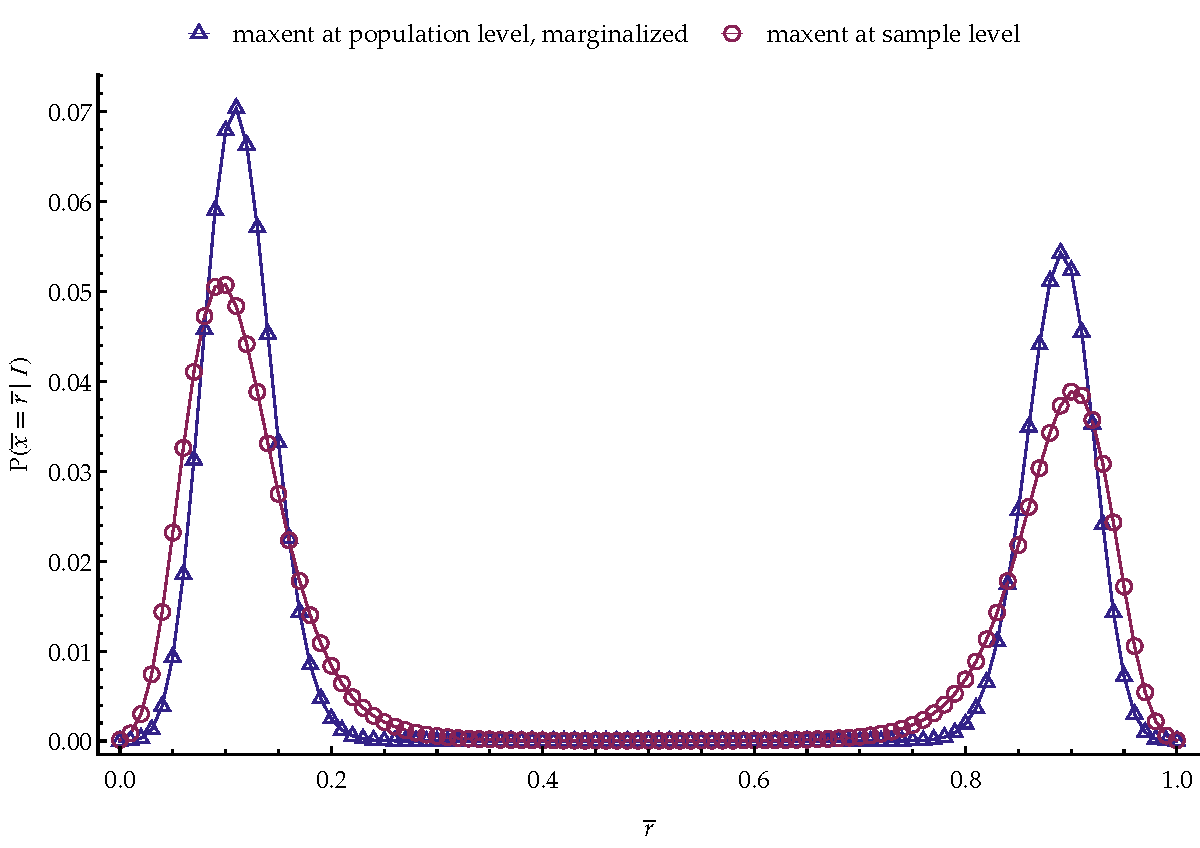
\includegraphics[width=0.99\linewidth]{different_maxent_pop_sample_100.pdf}%
\caption{Plots of $\p(\yxs = \yrs)$ constructed by \me\ at the population
  level followed by sample marginalization (blue triangles),
  \eqn~\eqref{eq:full_pop_av_example_ME_marg}, and at the sample level (red
  circles), \eqn~\eqref{eq:sample_av_example_ME}. In this case $N=5\,000$,
  $n=100$, $\expe{\yxs}=0.45$, $\expe{\yxxs}=0.35$, $\yL_1 = -13\,321.9$,
  $\yL_2 = 13\,321.5$, $\yl_1=-269.3$, $\yl_2 = 268.9$.}
\label{fig:diff_maxent_pop_sample}
\end{figure}%maxent_pop_or_sample.nb
% \end{wrapfigure}
\begin{figure}[!t]
\centering
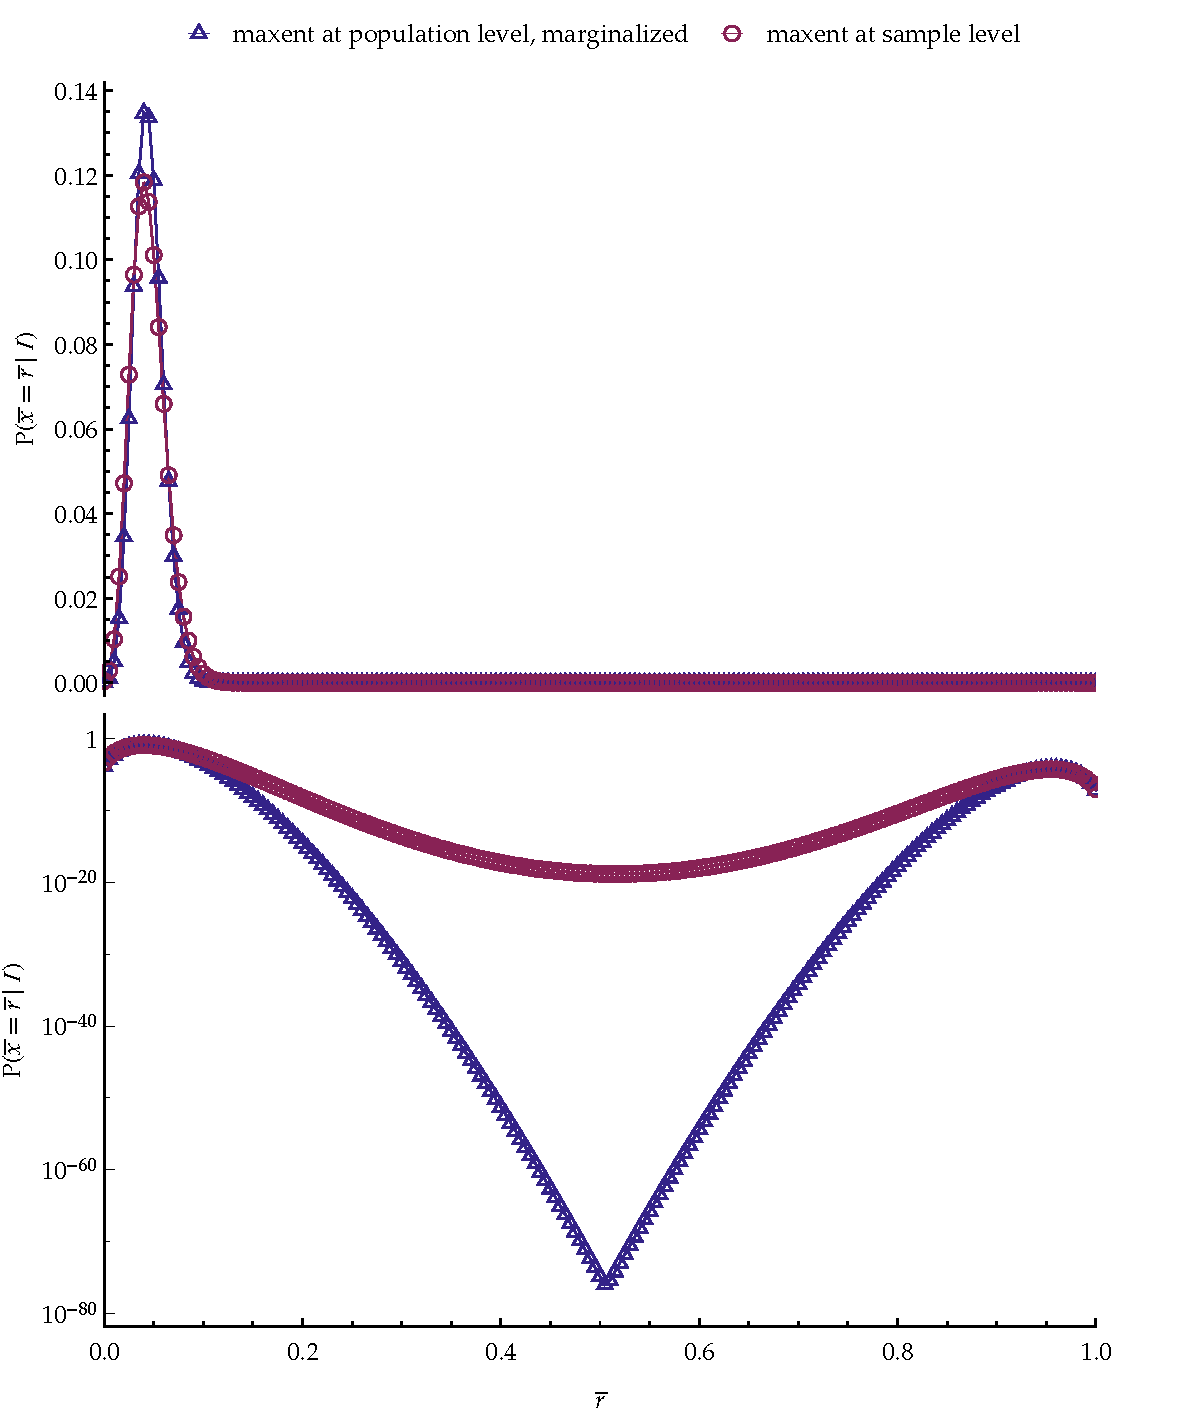
\includegraphics[width=0.99\linewidth]{different_maxent_pop_sample_200_realdata_both.pdf}
% 
\caption{Linear and log-plots of $\p(\yxs = \yrs)$ constructed by \me\ at
  the population level followed by sample marginalization (blue triangles),
  \eqn~\eqref{eq:full_pop_av_example_ME_marg}, and at the sample level (red
  circles), \eqn~\eqref{eq:sample_av_example_ME}. In this case $N=5\,000$,
  $n=200$, $\expe{\yxs}=0.045$, $\expe{\yxxs}=0.0025$,
  $\yL_1 = -16\,834.0$, $\yL_2 = 16\,825.7$, $\yl_1=-673.5$,
  $\yl_2 = 665.1$.}
\label{fig:diff_maxent_pop_sample_realdata}
\end{figure}%maxent_pop_or_sample.nb

The resulting distributions $\p(\yxs = \yrs \| \yHa)$,
$\p(\yxs = \yrs \| \yHb)$ are different.
Figure~\ref{fig:diff_maxent_pop_sample} shows one example, for $N=5\,000$,
$n=100$, $c_1=0.45$, $c_2=0.35$. The two distributions have slightly
different modes and the one obtained from \me\ at the population level is
more peaked. Another example is shown in
\fig~\ref{fig:diff_maxent_pop_sample_realdata}, for $N=5\,000$, $n=200$,
and neurobiologically more realistic constraints $c_1=0.045$, $c_2=0.0025$
\cite{rostamietal2016}. The discrepancy is maybe not as large as in the
previous example, but the tails of the distributions are still very
different.


The inequivalence of the two \me\ applications is generally valid for small
number of constraints, even if the two states of knowledge $\yHa$, $\yHb$
use different numbers $m'$, $m''$ \emph{and values} of constraints. The
equality $\p(\yxs = \yrs \| \yHa) = \p(\yxs = \yrs \| \yHb)$ in this case
requires solving $n$ equations in $m'+m''$ unknowns (normalization
is taken care of), so in general it can only be satisfied if $n\le m'+m''$.

\medskip

Where should we apply the \me\ method then, on the sample or on the
population?

\section{Discussion}
\label{sec:discussion}

We prefer not to answer the question that closed the preceding section,
because the optimal answer can only be given case by case, depending on the
inferences we are trying to make, on the assumptions needed and negligible,
and on our computational power. We would just like to stress that the
answer is not unique, and some answers may imply assumptions we were not
aware of.

The probability distribution for the sample average obtained by applying
\me\ at the population level has by construction a lower entropy than the
one obtained by application at the sample level. It says that some sample
states $\yx$ should be considered less likely than in the other
distribution. The lower entropy signals the presence of an additional
physical assumption behind the former distribution. Such assumption,
intuitively, is that the sample is part of a larger population, of which it
is representative. And this assumption may affect our predictions.
\mynote{It is a very natural assumption in the neuroscientific context and
  therefore we find it preferable. In fact, also physical neuronal network
  model add an external input to the neurons, mimicking their embedding in a
  larger network}

\iffalse
The quandary we found in the present note has at least two bright sides.
The first is that the two different \me\ applications may give numerically
similar results in some cases. One could thus be used as an approximation
of the other, depending on the circumstances -- \eg\ if probability tails
are unimportant. See \fig~\ref{fig:diff_maxent_pop_sample_realdata} for an
example.
\begin{figure}[!t]
\centering
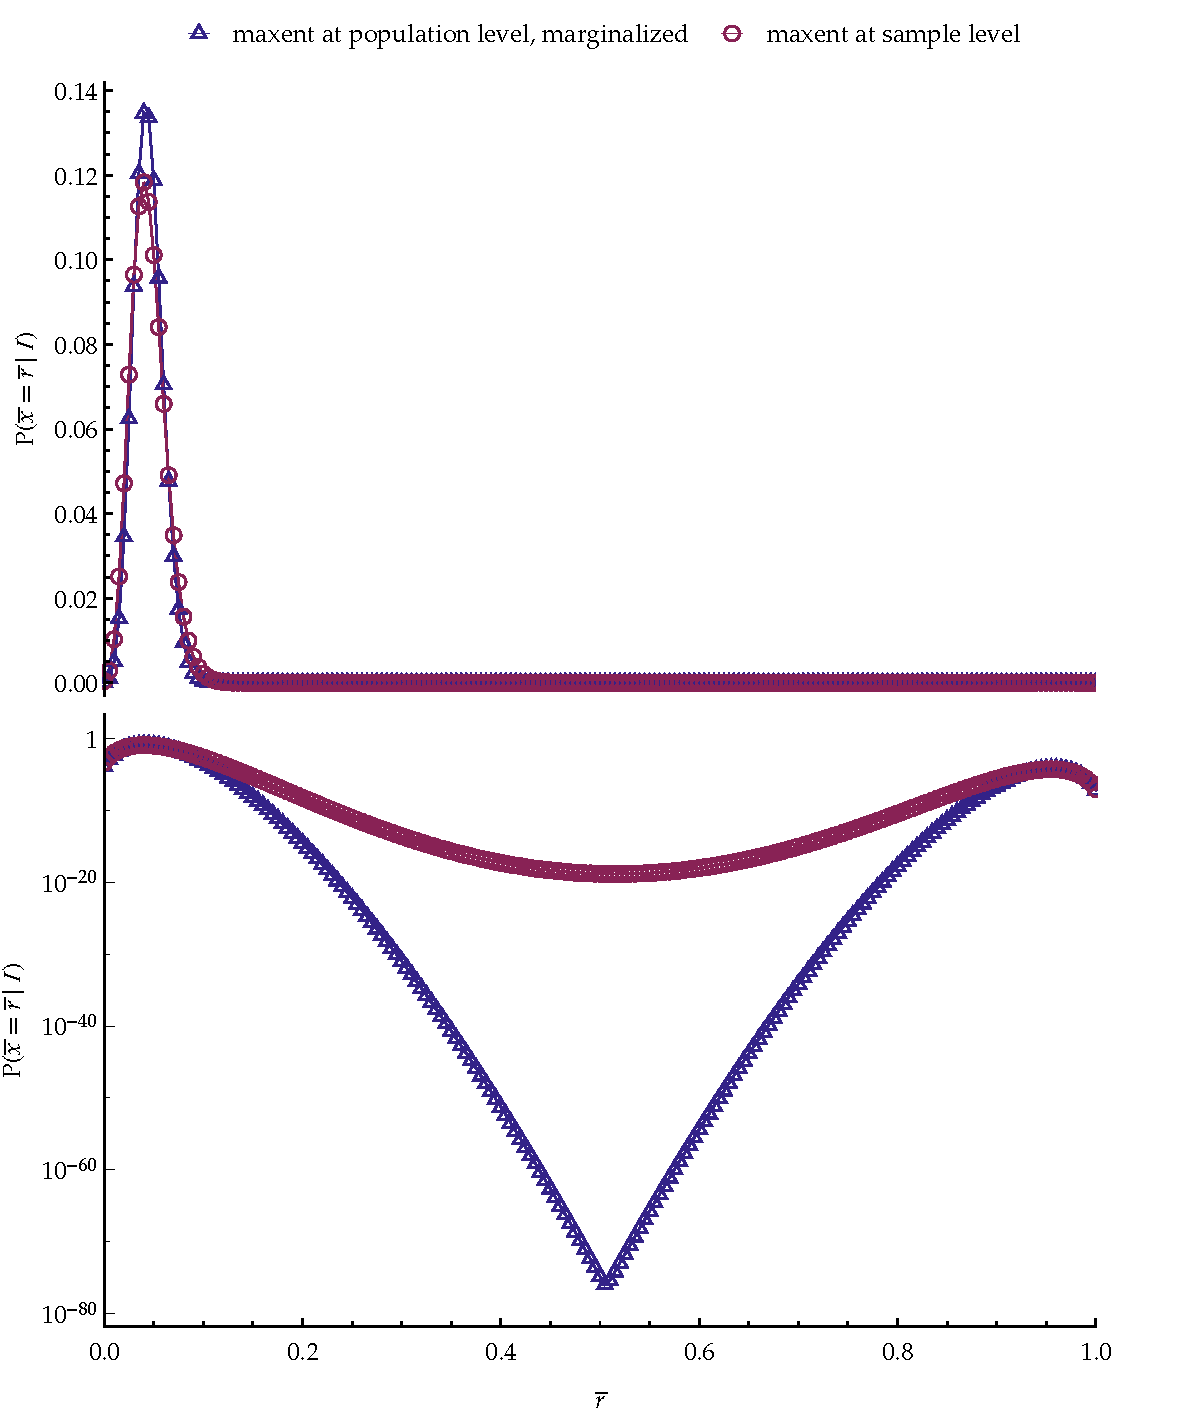
\includegraphics[width=0.95\columnwidth]{different_maxent_pop_sample_200_realdata_both.pdf}
% 
\caption{Example of discrepancy in $\p(\yxs = \yrs \| \yH)$ constructed by
  \me\ at the population level followed by sample marginalization (blue
  triangles), and at the sample level (red circles). The constraints are
  the same in either case: $\expe{\yxs \|\yH}=0.045$,
  $\expe{\yxxs \|\yH}=0.0025$, and $N=5\,000$, $n=200$.}
\label{fig:diff_maxent_pop_sample_realdata}
\end{figure}%maxent_pop_or_sample.nb
The second is that
\fi
The possibility of using two different distributions is
not a physical contradiction. Similar situations arise in statistical
mechanics. It is known that if a system is described by a \me\ Gibbs state,
its subsystems need not be \cite{maesetal1999}. A quandary somehow similar
to ours also appears in the statistical description of an equilibrium state
at the end of a non-equilibrium process: we can describe our knowledge
about it either by a Gibbs distribution, or by the Liouville-evolved Gibbs
distribution associated with equilibrium state at the beginning of the
process. The two descriptions differ -- even though the final physical
state is exactly the same \cite[\sect~4]{jaynes1985d_r1993}. The appearance
of this difference is natural: in one case we can make sharper predictions
about the state thanks to our knowledge of its preceding dynamics.
\mynote{but in this case both distributions are immensely sharp, and this
  doesn't affect predictions}

\mynote{Importance of the formulae relating sample and population.}

\mynote{Discussion of case when individual $X_i\dotsm X_j$ are constrained.
Likely breakdown of \me\ in this case \cite{portamana2009}. Hints at full
Bayesian treatment of which \me\ is a limit? \cite[***]{mackay1995_r2003}}


% do not change font sizes (except perhaps in the \textbf{References}
% section; see below).


\subsubsection*{Acknowledgments}

PGLPM thanks Mari \amp\ Miri for continuous encouragement and affection,
Buster Keaton for filling life with awe and inspiration, and the developers
and maintainers of \LaTeX, Emacs, AUC\TeX, MiK\TeX, arXiv, biorXiv,
PhilSci, Hal archives, Python, Inkscape, Sci-Hub for making a free and
unfiltered scientific exchange possible.

% Use unnumbered third level headings for the acknowledgments. All
% acknowledgments go at the end of the paper. Do not include
% acknowledgments in the anonymized submission, only in the final paper.

%\section*{References}
\renewcommand*{\bibname}{References}
\defbibheading{bibliography}[\bibname]{\section*{#1}\addcontentsline{toc}{section}{#1}%\markboth{#1}{#1}
}

% References follow the acknowledgments. Use unnumbered first-level
% heading for the references. Any choice of citation style is acceptable
% as long as you are consistent. It is permissible to reduce the font
% size to \verb+small+ (9 point) when listing the references. {\bf
%   Remember that you can go over 8 pages as long as the subsequent ones contain
%   \emph{only} cited references.}
% \medskip

% \small

% [1] Alexander, J.A.\ \& Mozer, M.C.\ (1995) Template-based algorithms
% for connectionist rule extraction. In G.\ Tesauro, D.S.\ Touretzky and
% T.K.\ Leen (eds.), {\it Advances in Neural Information Processing
%   Systems 7}, pp.\ 609--616. Cambridge, MA: MIT Press.

% [2] Bower, J.M.\ \& Beeman, D.\ (1995) {\it The Book of GENESIS:
%   Exploring Realistic Neural Models with the GEneral NEural SImulation
%   System.}  New York: TELOS/Springer--Verlag.

% [3] Hasselmo, M.E., Schnell, E.\ \& Barkai, E.\ (1995) Dynamics of
% learning and recall at excitatory recurrent synapses and cholinergic
% modulation in rat hippocampal region CA3. {\it Journal of
%   Neuroscience} {\bf 15}(7):5249-5262.
\defbibnote{postnote}{\small\par\medskip\noindent{\footnotesize% Note:
\arxivp \mparcp \philscip \biorxivp}%
}

\newcommand*{\citein}[2][]{\textnormal{\textcite[#1]{#2}}%\addtocategory{extras}{#2}
}
\newcommand*{\citebi}[2][]{ref.\ \citep[#1]{#2}%\addtocategory{extras}{#2}
}
\newcommand*{\subtitleproc}[1]{}


\printbibliography[postnote=postnote]

\newrefsection
\bigskip
{\centering\mynote{*** From here down old text to be discarded ***}\par}
\section{***}

\iffalse
\begin{align}
  \expe{x_{i_1} \dotsm x_{i_m} \| \yH}
&=
\expe{\sav{\underbrace{\yx \dotsm \yx}_{\text{$m$ factors}}} \| \yH}
=
\expe{\av{\underbrace{\yX \dotsm \yX}_{\text{$m$ factors}}} \| \yH},
\\
\intertext{and has an explicit expression in terms of $Q$:}
  \begin{split}
\expe{x_{i_1} \dotsm x_{i_m} \| \yH}
&=
\binom{N}{m}^{-1}
%\frac{(N-m)!}{N!}
\sum_{N A=0}^N %m!\, 
\binom{N A}{m}\, Q(A)
\\
&\equiv
%\frac{(N-m)!}{N!}
\sum_{N A=0}^N %m!\, 
\binom{N-m}{N A-m}
\binom{N}{N A}^{-1} Q(A).
\end{split}
\end{align}
\end{subequations}
\fi


What do we mean by saying that we can learn something about the population
by observing the sample? At the very least we mean that our uncertainty
about the rest of the population can change upon observing the sample. That
is, the probability for the state $\yy$ of the rest of the population is
conditionally dependent on the sample's values:
\begin{equation}
  \label{eq:conditionally_dependent_sample}
  \p(\yy =\ys \| \yx=\yr,\yH) \ne \p(\yy =\ys \|\yH)
  \qquad\text{for some $\ys,\yr$},
\end{equation}
This also means that the probability for the population cannot be
factorized into that of the sample times that of the complement.

What do we mean when we say that the sample is representative of the
population? It means that we expect some collective properties of the
sample, like the fraction of active neurons, or the fraction of
simultaneously active pairs, to be roughly equal to those of the full
population.

***

For example, $\yX$ can
represent the state of a population at a particular time. We call the
neurons \enquote{units} to lend some generality to our discussion. We shall
make statements about the whole population of $N$ units and about a
subpopulation of $n$ units; the word \enquote{population} will always refer
to the \emph{whole} population. The subpopulation states and their values
are denoted by lowercase letters: $(x_1, \dotsc, x_n)\equiv\yx$ and
$(r_1, \dotsc, r_n)\equiv\yr$; but note that $x_i \equiv X_{j_i}$ and
$r_i \equiv R_{j_i}$ for some distinct $j_1,\dotsc,j_n$. We shall also make
statements about the population-averaged state, or \emph{population
  average}:
\begin{align}
  \label{noeq:population-av}
   \yXf &\defd (X_1 + \dotsb + X_N)/N,
\\
\intertext{and the subpopulation-averaged state, or \emph{subpopulation average}:}
\label{noeq:subpopulation-av}
\yxs &\defd (x_1 + \dotsc + x_n)/n.
\end{align}
The quantities $N\yXf$ and $n\yxs$ represent the total number of active
units in the population and the subpopulation. Quantities like $\yRf$ and $\yrs$
are defined analogously. The averaging operators $\sav{\dotv}$ and
$\av{\dotv}$ are also extended to averages of $\tbinom{n}{m}$ or
$\tbinom{N}{m}$ products of $m$ states; \eg,
\begin{align}
\av{\yX \yX} &\defd
\tbinom{N}{2}^{-1} (X_1 X_2 + X_1 X_3  + \dotsb +  X_{N-1} X_N),
\\[2\jot]
\sav{\yx\yx\yx} &\defd
\tbinom{n}{3}^{-1} (x_1 x_2 x_3 + x_1 x_2 x_4 + \dotsb + x_{n-2} x_{n-1} x_n),
\end{align}
and so on.


\subsection{Assumptions}
\label{nosec:assumptions}

Our uncertainty about the population state is represented by the joint
probability distribution of the individual states, from which we can
derive all other probabilities of interest. We denote it by
\begin{equation}
  \label{noeq:joint_plaus}
  \p(X_1=R_1, X_2=R_2, \dotsc, X_N=R_N \| \yH) \quad\text{or}\quad
\p(\yX =\yR \| \yH).
\end{equation}
Such probability is conditional on our state of knowledge, \ie\ the
evidence and assumptions backing our probability assignments, denoted by
the proposition $\yH$.

In the present discussion, $\yH$ is a state of knowledge that leads to two
specific properties in our probability assignments:

\medskip
\begin{enumerate}%[wide,label=$\yH$\arabic*.]
\item \emph{Permutation symmetry}, expressed as the invariance of the
  joint distribution~\eqref{noeq:joint_plaus} under arbitrary permutations of
  the units's labels:
\begin{multline}
  \label{noeq:homog_math}
  \p(X_1=R_1, X_2=R_2, \dotsc, X_N=R_N \| \yH) ={}
\\ 
\shoveright{\p(X_1=R_{\pi(1)}, X_2=R_{\pi(2)}, \dotsc, X_N=R_{\pi(N)} \| \yH)}
\\
\text{for any permutation $\pi$}.
\end{multline}
This property can reflect two very different states of knowledge: physical
homogeneity of the population, or symmetry in our ignorance about the population.
This property is called \emph{finite exchangeability} in the Bayesian
literature and its basis, consequences, and alternatives to it are discussed
in \sect~***%\ref{nosec:stoch_symm}.

\medskip

\item The population average $\yXf$ has a particular distribution $Q$:
\begin{equation}
  \label{noeq:pop_average_Q}
  \p(\yXf = A \| \yH)
% \equiv \pr(x_1+ \dotsb + x_N = N A \| \varEta) 
=  Q(A),
\qquad
A \in \set*{0,\tfrac{1}{N},\tfrac{2}{N},\dotsc,1}.
\end{equation}
For the moment we are not concerned about the specific form of $Q$ and
about how it was assigned: it could, \eg, arise from maximum-entropy
arguments
\citep[\eg:][]{jaynes1957,jaynes1963,good1963,jaynes1967,aczeletal1975,jaynes1979b,vancampenhoutetal1981,sivia1990,fangetal1997,bretthorst2013}
used with data on the population.
\end{enumerate}

\subsection{Formulae}
%\section{\ding{41} {\itshape The mathematical relations} \ding{41}}
%\section*{3.\hspace{\stretch{1}}The mathematical relations\hspace{\stretch{1}}\mbox{}}
%\addcontentsline{toc}{section}{The mathematical relations}
\label{nosec:main_formulae}

The state of knowledge $\yH$ has the following six (not independent) main
consequences for our probability assignments:

\begin{enumerate}%[wide,label=\textbf{\emph{\Roman*}}.]
  \medskip\item\label{noitem:tot_plaus}Probability for the population state:
\begin{equation}
  \label{noeq:joint_plaus_N_homog}
  \p(\yX = \yR \| H) = \binom{N}{N\yRf}^{-1} Q(\yRf).
\end{equation}

\medskip
\item\label{noitem:marginal}Probability for the state $\yx$ of any subpopulation
  of $n$ units:
\begin{equation}
  \label{noeq:marginal}
    \p(\yx = \yr \| \yH) =
\sum_{N A =0}^{N} 
\binom{N-n}{N A-n\yrs}\binom{N}{N A}^{-1}\,
Q(A).
\end{equation}
Note that the only summands contributing to this sum are those for which
$n\yrs \le NA \le N$; the others are zero because by definition
$\tbinom{M}{y}=0$ if $y<0$. This remark applies to all the sums of this
kind in the rest of this Note.

\medskip
\item\label{noitem:conditional}Probability for the subpopulation
  state conditional on a population state:
\begin{equation}
  \label{noeq:conditional_total_state}
  \p(\yx = \yr \| \yX = \yR, \yH)
=
\binom{N-n}{N \yRf-n \yrs}.
\end{equation}

\medskip
\item\label{noitem:marginal_average}Probability for the
  subpopulation average $\yxs$:
\begin{multline}
  \label{noeq:subpop_average}
  \p(\yxs = a  \| \yH) = \binom{n}{n a}
 \sum_{N A=0}^{N}
\binom{N-n}{N A-n a}\binom{N}{N A}^{-1}\,
Q(A),
\\
a \in \set*{0,\tfrac{1}{n},\tfrac{2}{n},\dotsc,1}.
\end{multline}

\medskip
\item\label{noitem:conditional_average}Probability for the subpopulation
  average conditional on the population average:
\begin{equation}
  \label{noeq:conditional_prob}
  \p(\yxs = a \| \yXf = A, \yH)
=
\binom{n}{n a}\binom{N-n}{N A-n a}\binom{N}{N A}^{-1}.
\end{equation}

\medskip
\item\label{noitem:moments}The product of the states of any $m$ distinct
  units from a given subpopulation,
  \begin{equation*}
    x_{i_1} x_{i_2} \dotsm x_{i_m},
    \qquad 1\le i_1 < i_2 < \dotsb < i_m \le n
  \end{equation*}
  has an expectation equal to that of the subpopulation average of such
  products, is independent of the subpopulation size $n$:
\begin{subequations}
\label{noeq:expe_products}
\begin{align}
  \expe{x_{i_1} \dotsm x_{i_m} \| \yH}
&=
\expe{\sav{\underbrace{\yx \dotsm \yx}_{\text{$m$ factors}}} \| \yH}
=
\expe{\av{\underbrace{\yX \dotsm \yX}_{\text{$m$ factors}}} \| \yH},
\\
\intertext{and has an explicit expression in terms of $Q$:}
  \begin{split}
\expe{x_{i_1} \dotsm x_{i_m} \| \yH}
&=
\binom{N}{m}^{-1}
%\frac{(N-m)!}{N!}
\sum_{N A=0}^N %m!\, 
\binom{N A}{m}\, Q(A)
\\
&\equiv
%\frac{(N-m)!}{N!}
\sum_{N A=0}^N %m!\, 
\binom{N-m}{N A-m}
\binom{N}{N A}^{-1} Q(A).
\end{split}
\end{align}
\end{subequations}
\end{enumerate}

\medskip


A useful relation connects the expectation of a
product~\eqref{noeq:expe_products} and the $m$th \emph{factorial moment}
\citep{potts1953} of the probability distributions for the averages. The
$m$th factorial moment of the subpopulation average $\yxs$ is defined by
\begin{equation}
  \label{noeq:fact_mom_defin}
\vphantom{\underbrace{\yxs}_{m}}\expeb*{
\smash{\underbrace{n\yxs\,(n\yxs-1)\dotsm \bigl(n\yxs-(m-1)\bigr)}_{\text{$m$ factors}}}
\| \yH}
\equiv \expeb*{\frac{(n\yxs)!}{(n\yxs-m)!} \| \yH},
\end{equation}
an analogous definition holding for $\yXf$. We have that
\begin{equation}
  \label{noeq:eq_factmom_prod}
\expe{x_{i_1} \dotsm x_{i_m} \| \yH}
=
  \tfrac{(n-m)!}{n!}\expeb*{\frac{(n\yxs)!}{(n\yxs-m)!} \| \yH}
=
  \tfrac{(N-m)!}{N!}\expeb*{\frac{(N\yXf)!}{(N\yXf-m)!} \| \yH}.
\end{equation}


As a consequence of the above relation, the first three moments of the
probability distributions $\p(\yxs=a\|\yH)$ and $\p(\yXf=A\|\yH)$,
are related by
\begin{subequations}\label{noeq:moments}
  \begin{align}
    \expe{\yxs \| \yH} &= \expe{\yXf \| \yH},
    \\[2\jot]
    \begin{split}
    \expe{\yxs^2 \| \yH} &= \expe{\yXf \| \yH}
                                  \frac{N-n}{(N-1)n}
 +{}
\\&\quad\quad \expe{\yXf^2 \| \yH}\frac{N\,(n-1)}{(N-1)n},
\end{split}
    \\[2\jot]
    \begin{split}
    \expe{\yxs^3 \| \yH} &=
                              \expe{\yXf \| \yH}\frac{(N-n)(N-2n)}{(N-1)(N-2)n^2}+{}
                                    \\
                                    &\quad\quad\expe{\yXf^2 \| \yH}
                                    \frac{3N\,(N-n)(n-1)}{(N-1)(N-2)n^2} +{}
                                    \\
                                    &\quad\quad\quad\expe{\yXf^3 \| \yH}
                                    \frac{N^2\,(n-1)(n-2)}{(N-1)(N-2)n^2}.
                                  \end{split}
                                    % \\[2\jot]
                                    % \expe{\yxs^4 \| \varEta} &=
                                    % \!\begin{aligned}[t] &\expe{\yxf
                                    %   \| \varEta}
                                    %   \frac{(N-n)(N^2+N-6Nn+6n^2)}{(N-1)(N-2)(N-3)n^3}+{}
                                    %   \\%[1.5\jot]
                                    %   &\quad\expe{\yxf^2 \| \varEta}
                                    %   \frac{(7N-11n+1)(N-n)(n-1)N}{(N-1)(N-2)(N-3)n^3}+{}
                                    %   \\
                                    %   &\quad\expe{\yxf^3 \| \varEta}
                                    %   \frac{6(n-1)(n-2)(N-n)N^2}{(N-1)(N-2)(N-3)n^3}
                                    %   +{}
                                    %   \\
                                    %   &\quad\expe{\yxf^4 \| \varEta}
                                    %   \frac{(n-1)(n-2)(n-3)N^3}{(N-1)(N-2)(N-3)n^3}.
                                    % \end{aligned}
  \end{align}
\end{subequations}
Relations for higher moments can be obtained recursively from
\eqn~\eqref{noeq:eq_factmom_prod}. In general, this means that the two sets of
first $m$ moments are related by a homogeneous linear transformation,
\begin{equation}
  \label{noeq:lin_transf_moments}
  \expe{\yxs^m \| \yH} = \sum_{l=1}^m M_{ml}(n,N) \expe{\yXf^l \| \yH},
\end{equation}
with a universal, lower-triangular transformation matrix $M_{ml}(n,N)$ that
depends only on $n$, $N$, and the condition of symmetry~\eqref{noeq:homog_math}.

As intuition suggests, we have 
%$\expe{\yxs^m \| \yH} \xrightarrow{n\to N} \expe{\yXf^m \| \yH}$.
\begin{equation}
  \label{noeq:limit_moments}
  \expe{\yxs^m \| \yH} \xrightarrow{n\to N} 
  \expe{\yXf^m \| \yH},
\qquad
  \expe{\yxs^m \| \yH} \xrightarrow{n\to 1} 
  \expe{\yXf \| \yH},
\end{equation}
the latter because ${x_i}^m=x_i$, since states are $\set{0,1}$-valued.

\bigskip

The core of the six mathematical relations above are
\eqns~\eqref{noeq:marginal} and~\eqref{noeq:subpop_average}. The latter
expresses the probability for the subpopulation average as a mixture of
hypergeometric distributions
\cites[\chap~3]{jaynes1994_r2003}[\sect~4.8.3]{ross1976_r2010}[\sect~II.6]{feller1950_r1968},
with parameters $N,N\yXf,n$, weighted by the probabilities
$\p(\yXf = A \|\yH)$ \citep[\cf][\sect~4, esp.\ \eqn~(22)]{kendall1967}.
The connection between this mixture representation and the condition of
symmetry~\eqref{noeq:homog_math} is well-known in the Bayesian literature
\citep{kendall1967,definetti1969b,heathetal1976,diaconis1977,diaconisetal1980,jaynes1986c}.


\section{Examples of inferential use of the formulae}

\subsection{From network to subnetwork}
\label{nosec:pop2sub_examples}


Let us illustrate with an example how the probability distribution for the
subnetwork average $\yxs$, determined by \eqn~\eqref{noeq:subpop_average},
changes with the subnetwork size $n$. Choose a network-average distribution
$\p(\yXf=A\| \yH)$ belonging to the exponential family
\cites[\sect~4.5.3]{bernardoetal1994}[see also][]{fortinietal2000}:
\begin{equation}
  \label{noeq:full_pop_av_example_ME}
  \p(\yXf = A \| \yH) = Q(A) \propto
\binom{N}{N A}\exp[
\yl_2\, N A\,(N A-1)/2 + \yl_1\, N A].
\end{equation}
This is the form obtained from the principle of maximum relative entropy
\citep[\eg:][]{jaynes1957,jaynes1963,good1963,jaynes1967,aczeletal1975,jaynes1979b,vancampenhoutetal1981,sivia1990,fangetal1997,bretthorst2013}
with first and second moments as constraints and the reference distribution
$Q_0$ defined by $Q_0(A) = 2^{-N}\binom{N}{N A}$, corresponding to a
uniform probability distribution for the network state $\yX$.
%file: distr_scaling_from_full_population.nb
\begin{figure}[!b]
\centering
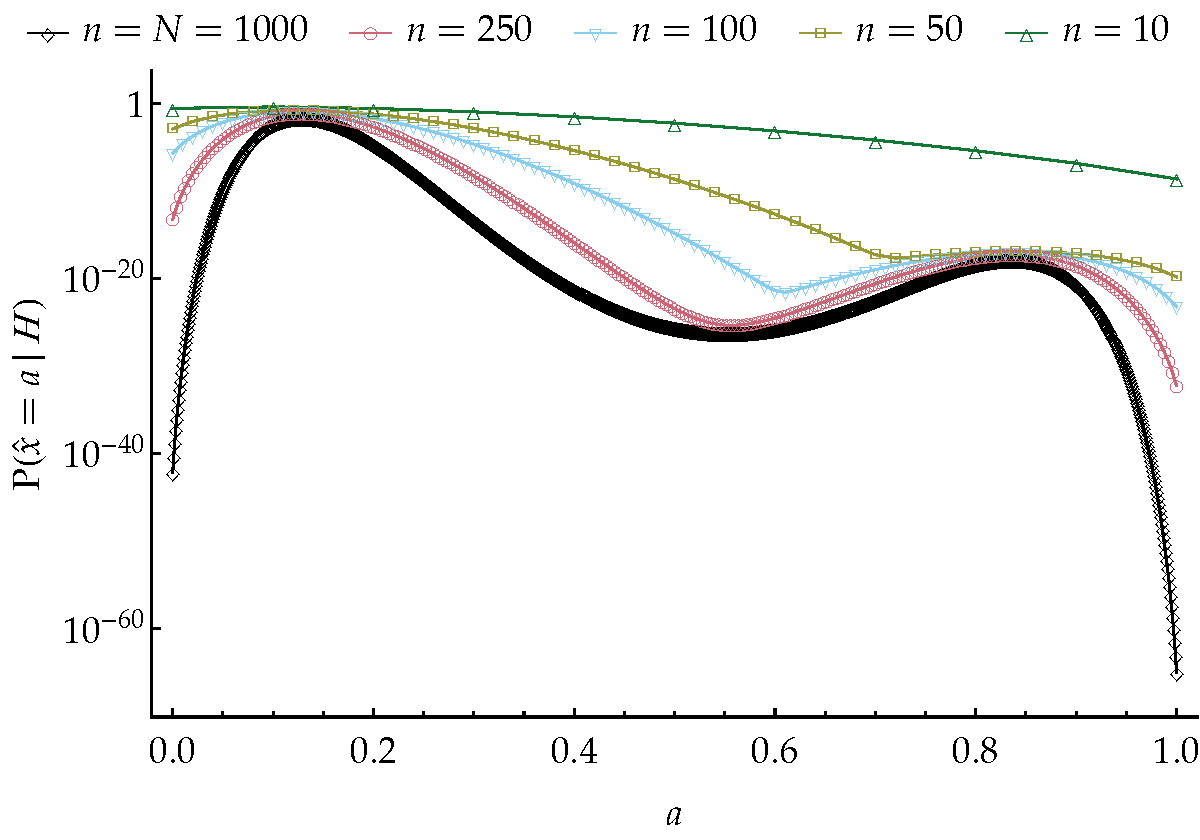
\includegraphics[width=0.95\columnwidth]{scaled_subpop_probs.pdf}%
\caption{Probability distributions $\p(\yxs = a \| \yH)$ for different
  subnetwork sizes $n$, obtained from a network probability
  distribution $\p(\yXf = A \| \yH)$ having the maximum-etropy
  form~\eqref{noeq:full_pop_av_example_ME}.}
\label{noscaling_distr}
\end{figure}
\begin{figure}[!b]
\centering
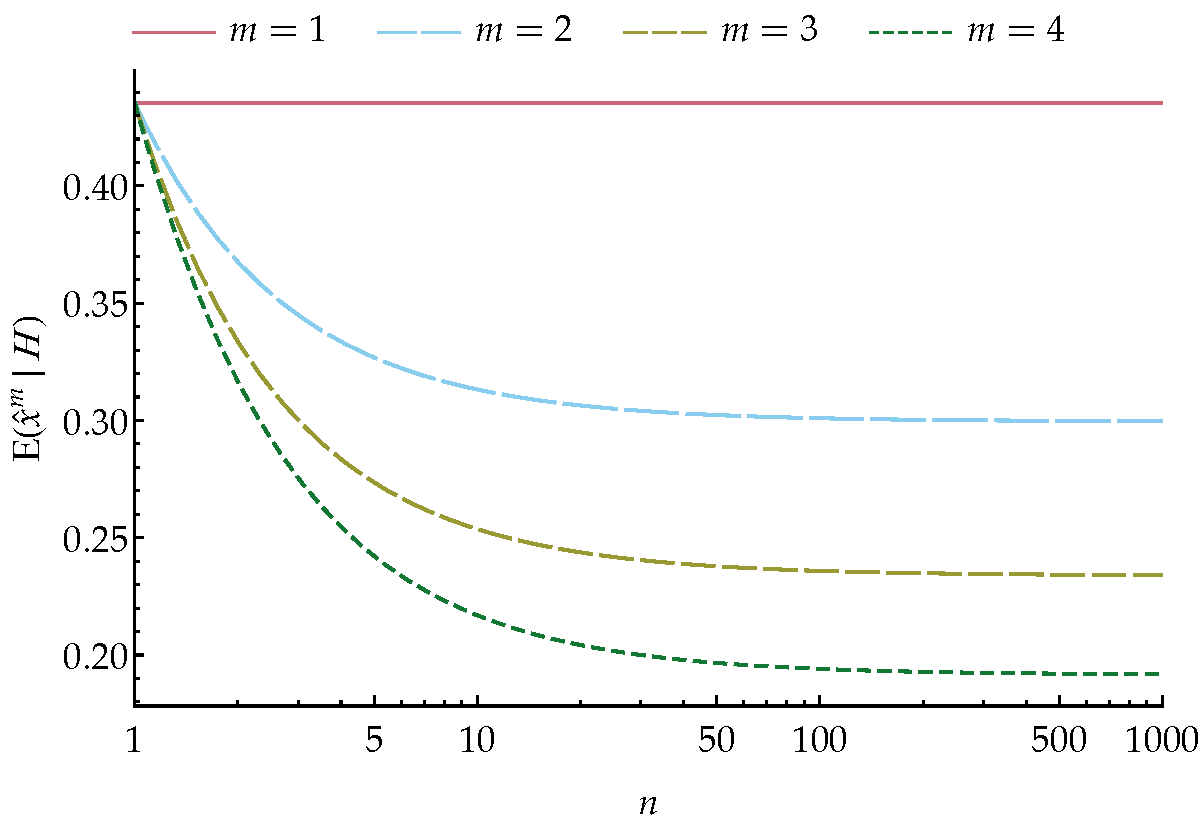
\includegraphics[width=0.95\columnwidth]{scaling_subpop_moments.pdf}%
\caption{Moments of the probability distributions $\p(\yxs =a \|
  \yH)$ as functions of the subnetwork size $n$.}
\label{noscaling_moments}
\end{figure}

The probability distribution of \eqn~\eqref{noeq:full_pop_av_example_ME} is
plotted in \fig~\ref{noscaling_distr}, together with the resulting
subnetwork-average distributions $\p(\yxs = a \|\yH)$, for the case in
which $N = 1000$ units, $\lambda_1=-2.55$, $\lambda_2=0.005$, and
$n=10, 50, 100, 250$. The distributions become broader as $n$ decreases,
and the minimum of the original distribution disappears; at the same time
the finite-difference 
\[\frac{\p(\yxs=a+1/n\|\yH)-\p(\yxs=a\|\yH)}{1/n}\]
presents a sharp jump at this minimum when $n\approx 100$.

To the eye familiar with maximum-entropy distributions, the
subnetwork-average distributions of \fig~\ref{noscaling_distr} do not look
like maximum-entropy ones with second-moment constraints. In fact,
they are not and \emph{cannot} be:
\begin{equation}
  \label{noeq:maxent_form_sub}
  \p(\yxs =a  \| \yH)
\ne\kappa\binom{n}{n a}\exp[\yk_2\, n a\,(n a-1)/2 + \yk_1\, n a]
%\quad\text{(false)}
\end{equation}
for any $\kappa, \yk_1, \yk_2$, unless $n=2$. This impossibility holds more
generally for any number of constraints $m$ and subnetwork size $n$ such
that $m<n$. The reason is simple: suppose we have assigned a
maximum-entropy distribution with $m$ moment constraints as the
distribution for the network average. If we want the same kind of
distribution for a subnetwork of size $n$, we are free to play with $m+1$
parameters (normalization included), but we must also satisfy the $n+1$
equations corresponding to the marginalization~\eqref{noeq:subpop_average}.
This is generally impossible unless $m \ge n$. (Impossibilities of a
similar kind appear in statistical mechanics, see \eg\
ref.~\citep{maesetal1999}.)
%file: test_ME_same_under_scaling.nb

This fact can be significant for recent works
\citep[\eg,][]{schneidmanetal2006,shlensetal2006,tkaciketal2006,marreetal2009,tkaciketal2009,ganmoretal2011,shimazakietal2012,tkaciketal2013,shimazakietal2015}
in which a maximum-entropy probability distribution with second- or
third-moment constraints is assigned to relatively small subnetworks
($n < 200$) of neurons. If we assume that such subnetwork is part of a
larger network, and assume the condition of symmetry~\eqref{noeq:homog_math},
then the larger network \emph{cannot} be assigned a maximum-entropy
distribution with the same number of constraints. Vice versa, if we assign
such a maximum-entropy distribution to the larger network, then none of its
subnetwork of enough large size $n$ can be assigned a similar
maximum-entropy distribution. See ref.~\citep{rostamietal2016} for a
broader discussion of this fact and of its consequences.

\medskip

The dependence of the first four moments $\expe{\yxs^m \| \yH}$ as a
function of size $n$ is shown in \fig~\ref{noscaling_moments}. The moments
become practically constant when $n \approx 100$ or larger. The
expectations of $m$-tuple products of states
$\expe{x_{i_1}\dotsm x_{i_m} \| \yH}$, proportional to the factorial
moments, are not shown as they do not depend on $n$.


\subsection{From subnetwork to network}
\label{nosec:from_sub_to_full}

We have seen that, given the condition of symmetry~\eqref{noeq:homog_math},
the probability $\p(\yXf = A \|\yH)$ for the network average determines
that of each subnetwork average, $\p(\yxs \|\yH)$, by the
marginalization \eqn~\eqref{noeq:subpop_average}. The reverse is trivially
not true, since \eqn~\eqref{noeq:subpop_average}, as a linear mapping from
$\RR^{N+1}$ to $\RR^{n+1}$, with $N$ larger than $n$, is onto but not into.
Assigning a probability distribution $\p(\yxs = a \|\yH)$ to a
subnetwork average $\yxs$ does not determine a network distribution
$\p(\yXf = A\|\yH)$: it only restricts the set of possible ones; this
set can in principle be determined via linear-programming methods
\citep{hailperin1965,hailperin1984,hailperin1996,hailperin2006,hailperin2011}.
\begin{innote}
  Analogous situations appear in the truth-valued logical calculus: if the
  composite proposition $\varAlpha\limplies \varBeta$ is assigned the
  truth-value \enquote{true}, then assigning $\varAlpha$ the value
  \enquote{true} also determines the value of $\varBeta$, whereas assigning
  $\varBeta$ the value \enquote{true} leaves the value of $\varAlpha$
  undetermined.
\end{innote}
The same linear-programming methods show that any inference from subnetwork
properties to network ones must necessarily start from some assumptions
$\varIota$ that assign a probability distribution
$\p(\yX = \yR \| \varIota)$ for the network states. The approaches to
this task and reformulations of it have become uncountable: they include
exchangeable models, parametric and non-parametric models, hierarchical
models, general linear models, models via sufficiency, maximum-entropy
models, and whatnot
\citep[\eg:][]{jeffreys1931_r1973,jeffreys1939_r2003,jaynes1994_r2003,bernardoetal1994,gelmanetal1995_r2014,ghoshetal1997,kallenberg2005,gregory2005,sivia1996_r2006,ferreiraetal2007,dawid2013,damienetal2013}.
We now show two examples, based on a maximum-entropy approach, that to our
knowledge have not yet been explored in the neuroscientific literature. For
a concrete application see \citep{rostamietal2016b}.



\paragraph{First example: moment constraints for the network.}
\label{nosec:maxent_moments}
Consider a state of knowledge $\yHa$ leading to the following properties:
\begin{enumerate}%[$\yHa$1.]
\item the expectations of the single and pair averages $\yxs$ and
  $\sav{\yx\yx}$ of a particular subnetwork have given values
  \begin{equation}
    \label{noeq:constr_ex1}
    \expe{\yxs \| \yHa} = c_1, \qquad \expe{\sav{x_i x_j}\|\yHa} = c_2;
  \end{equation}
\item the network probability distribution $\p(\yX = \yR \|\yHa)$
  has maximum relative entropy with respect to the uniform one, given the
  constraints above.
\end{enumerate}

\medskip Then the probability distribution for the network conditional on $\yHa$
is completely determined: it satisfies the symmetry
property~\eqref{noeq:homog_math} and is defined by
\begin{multline}
  \label{noeq:pop_distr_maxent1}
  \pf(\yX =\yR \|\yHa) =
\varKappa\exp[\yL_2 N\yRf\,(N\yRf-1)/2 + \yL_1 N\yRf]
\\
\!\begin{aligned}[b]
&\text{with $\varKappa, \yL_m$, such that the distribution is normalized and}
\\
&\varKappa\sum_{N A=0}^N %m!\, 
\binom{N-m}{N A-m}
\exp[\yL_2 N A\,(N A-1)/2 + \yL_1 N A]
= c_m, \quad m=1,2.
\end{aligned}
\end{multline}
We omit the full proof of this statement: it is a standard application of
the maximum-entropy procedure
\citep[\eg:][]{jaynes1957,jaynes1963,good1963,jaynes1967,jaynes1979b,vancampenhoutetal1981,sivia1990,fangetal1997,bretthorst2013},
combined with the equality~\eqref{noeq:expe_products} of subnetwork and
network expectations, \eg
\begin{equation}
  \label{noeq:exploit_eq_expects}
  c_2 = \expe{\sav{\yx\yx}\|\yHa} = 
\binom{N}{2}^{-1}
\sum_{N A=0}^N %m!\, 
\binom{N A}{2} \, \p(\yXf = A\|\yHa),
\end{equation}
and with relations~\eqref{noeq:joint_plaus_N_homog},
\eqref{noeq:conditional_total_state}. This example is easily generalized to
any number $m$ of constraints such that  $m\le n$.

Note again that, as remarked in \sect~\ref{nosec:pop2sub_examples}, the
subnetwork from which the averages in the
expectations~\eqref{noeq:constr_ex1} are calculated has a probability
distribution $\p(\yxs =a \|\yH)$ determined by the
marginalization~\eqref{noeq:subpop_average} and does \emph{not} have a
maximum-entropy form with the same number of constraints.
%file: test_ME_same_under_scaling.nb


\paragraph{Second example: subnetwork-distribution constraint.}
\label{nosec:maxent_fullsubpop}
Consider another state of knowledge $\yHb$ leading to the following
properties:
\begin{enumerate}%[wide,label=$\yHb$\arabic*.]
\item the average $\yxs$ of a particular
  subnetwork has a probability distribution $q$:
  \begin{equation}
    \label{noeq:constr_subpop_distr}
    \p(\yxs =a \|\yHb) = q(a);
  \end{equation}
\item the probability distribution for the network, $\p(\yX = \yR
  \|\yHb)$, has maximum relative entropy with respect to the uniform
  one, given the constraint above.
\end{enumerate}

\medskip Then the probability distribution for the network given $\yHb$ is
completely determined and satisfies the symmetry
property~\eqref{noeq:homog_math}:
\begin{multline}
  \label{noeq:pop_distr_maxent2}
  \p(\yX= \yR \|\yHb) =
\exp\Biggl[
\sum_{n a=0}^n \yL_{ a}
%\binom{N}{N\yXf}^{-1}
\binom{n}{n a}
\binom{N-n}{N\yRf-n a}\Biggr]
\\
\!\begin{aligned}[b]
&\text{with $\yL_{ a}$ such that}
\\
&\sum_{N A=0}^N 
%\binom{N}{N A}^{-1}
\binom{n}{n a}
\binom{N-n}{N A-n a}\,
\exp\Biggl[
\sum_{n a=0}^n \yL_{ a}
%\binom{N}{N A}^{-1}
\binom{n}{n a}
\binom{N-n}{N A-n a}\Biggr]
=q( a)
\end{aligned}
\end{multline}
(the normalization constraint being unnecessary since $q$ is normalized).
This result is just another application of the maximum-entropy procedure
with $n+1$ (linear) constraints given by \eqn~\eqref{noeq:marginal}, where
the left-hand side is now given and equal to $q(a)$.

This example is equivalent to the generalization of the previous one with
$n$ moment constraints, since knowledge of $\p(\yxs=a \| \yHb)$ is
equivalent to knowledge its first $n$ moments.

***



In this note we would like to analyse and warn about a subtle assumption
behind the \me\ method when it is applied to a population. It can informally
be put this way:
\begin{quote}
  \emph{the \me\ method assumes that the population it is applied to is
    completely isolated from any larger population.}
\end{quote}

\mynote{Version 1}
The \me\ method does not construct a probability distribution out of
nothing, but starting from a uniform distribution. A uniform distribution
is an innocuous assumption for a set of non-composite events, like the
outcomes of a die roll, and also for some sets of composite events, like
the outcomes of the roll of two dice. In the latter case multiplicities
appear.

When applied to a subpopulation, the \me\ method assumes that the uniform over
the larger population is uniform, and therefore factorizable. The new
distribution of the subpopulation will not be uniform, but that of the full
population will still be factorizable into the one for the subpopulation and the
rest.

A uniform distribution, however, is not the right one when we suppose that
learning about an event may tell us something about a related event. For
example, consider 1\,000 tosses of a particular coin and assume a uniform
distribution over the possible $2^{1\,000}$ outcomes. If we learn that the
first 999 tosses yielded all \enquote{heads}, the probability calculus
tells us that the probability for the 1\,000th toss is still 50\%/50\%. It
is a consequence of our choice of a uniform distribution: we have
implicitly declared all tosses to be completely independent, completely
\emph{irrelevant} to one another. This fact is well-known in sampling
theory. A more telling example in fact is that of a presidential election
with two candidates: each citizen will vote for one or the other. We do
survey sampling on a large number of citizens to guess the election's
outcome. If we assumed a uniform distribution over the possible
combinations of choices of all citizens, our sampling would be completely
irrelevant for the choices of the rest of the population.




The latter example has many similarities with that of a neuronal binary
population. When we record the neuronal activity of a sample of neurons from a
brain area, we assume that our measurements can tell us something -- no
matter how vague or imprecise -- about the whole brain area. This means
that we are not assuming a uniform distribution over all possible states of
the area.




\mynote{Version 2}
This may come as a surprise. The method simply requires a number of
exhaustive and mutually exclusive events, and if these are composite events
the final distribution may have a multiplicity factor. When we consider the
$2^{N}$ states of $N$ units we are not excluding that these might be
marginals of $2^{M}$ states of $M$ units. Each one has the same
multiplicity $2^{M-N}$, but this constant multiplicity factor disappears
by normalization. So the method applies just as in the case of $N$ units
only, right?

Right, but 

Right, and that is where the problem lies. This way of counting of
multiplicities assumes an underlying 

Wrong. In our reasoning we have made subtle assumptions of independence
between the full population and the subpopulation. The problem is that the
counting of multiplicities is not based on simple enumeration, but already
involves probability considerations. Consider three cases with a full
population of two units, $M=2$, of which we consider one unit, $N=1$.
\begin{itemize}
\item First case: all four states are \emph{possible}. The two states of
  the first unit have multiplicity $2$ each. The usual \me\ distribution
  obtains.
\item Second case: only the states with at most one active unit are
  possible. The state $\yxx_1=1$ of the first unit has multiplicity
  $2$, and $\yxx_1=1$ has multiplicity $1$. The \me\ distribution has
  multiplicity factors.
\item Third case: states with at most one active unit are, say, $10^{9}$
  times more probable than the state with no active units. But all four
  states are \emph{possible}. By enumeration this case is like the first:
  multiplicities $(1,1)$. But by common sense it is more similar to the
  second: multiplicities $(2,1)$ for most practical purposes.
\end{itemize}

This simple example shows that the multiplicity inspection that must
precede a \me\ application already involves probability considerations at
the level of the full population. The usual reasoning by enumeration
implicitly assumes a uniform distribution or at least a \emph{factorizable}
distribution.

***If the distribution is factorizable, however, it means that examination of
the subpopulation \emph{cannot give us any insights about the population it is a
  part of}. This is obviously contrary to the reason why we made neuronal observations.

Consider the following ways of proceeding. We:
\begin{enumerate}
\item have a population with $N$ units, $2^{N}$ possible states
\item expect averages of $\yx$ active neurons and $\yxxs$ active pairs
\item use maximum-entropy to choose a probability distribution for the
  states of the $N$ units conforming to our expectations.
\end{enumerate}

We:
\begin{enumerate}
\item have a population with $M$ units, $2^{M}$ possible states
\item expect that any subpopulation of $N$ units has $\yxs$ active
  neurons and $\yxxs$ active pairs
\item use maximum-entropy to choose a probability distribution for the
  states of the $M$ units conforming to our expectations
\item marginalize to find the probability distribution for the states of
  $N$ units.
\end{enumerate}



  \section{Sketched proofs}
  \label{nosec:derivations}

  Variants of the following derivations and combinatorial considerations
  can be found \eg\ in
  \cites[\chaps~I--IV]{whitworth1867_r1965}[\chap~II]{feller1950_r1968}[\chap~3]{jaynes1994_r2003};
  see also \citep{whitworth1897}.

  To derive the joint probability distribution
  \eqref{noeq:joint_plaus_N_homog} from that for the network
  average~\eqref{noeq:pop_average_Q}, consider that if the network total
  is $N\yXf$, then $N\yXf$ out of $N$ units are active, and there are
  $\tbinom{N}{N\yXf}$ possible states for which this can be true; therefore
  \begin{equation}
    \labelbis{eq:joint_plaus_N_homog}
    \p(\yX = \yR \| H) = \binom{N}{N\yRf}^{-1}Q(\yRf).
  \end{equation}
An analogous reasoning for $n$ and $\yxs$ leads to an analogous equality,
\begin{equation}
  \label{noeq:aver_subpop}
  \p(\yx=\yr \| H) = \binom{n}{n\yrs}^{-1} \p(\yxs=\yrs\|\yH),
\end{equation}
for the subnetwork.

\bigskip 

Let us next consider the probability $\p(\yxs =a \| \yXf = A,\yH)$ for
the subnetwork average $\yxs$ conditional on the network average $\yXf$.
There are $\tbinom{N}{N\yXf}$ possible network states if the network
average is $\yXf$, \ie\ if $N\yXf$ units are in state $1$; the conditional
probability of each is therefore $1/\tbinom{N}{N\yXf}$, owing to the
symmetry assumption~\eqref{noeq:homog_math}. Now consider the subnetwork of the
first $n$ units. The conditional probability of having $n\yxs$ specific
ones in state $1$ is the sum of the probabilities of all states for
which $N\yXf-n\yxs$ of the remaining $N-n$ units are in state $1$; there are
$\tbinom{N-n}{N\yXf-n\yxs}$ such states, all equally probable. Finally,
there are $\tbinom{n}{n\yxs}$ possible ways, all equally probable, in which
$n\yxs$ of the first $n$ units can be in state $1$. In formulae,
\begin{equation}
\label{noeq:conditional_prob_explained}
\begin{split}
      \p(\yxs =a \| \yXf=A, \yH)
      &=
      \sum_{\yr}^{\yrs=a} \sum_{\yR}^{\yRf=A} 
      \p(\yx =\yr \|  \yX = \yR, \yH) \,
      \p(\yX =\yR  \| \yXf=A,\yH),
      \\
      &=
      \sum_{\yr}^{\yrs=a} \sum_{\yR}^{\yRf=A} 
      \p(\yx=\yr \|  \yX =\yR, \yH) \,
      \binom{N}{N A}^{-1},
      \\
      &=\sum_{\yr}^{\yrs=a} 
      \binom{N-n}{N A-n a}\binom{N}{N A}^{-1},
      \\
      &=
      \binom{n}{n a}\binom{N-n}{N A-n a}\binom{N}{N A}^{-1},
\end{split}
\end{equation}
  which is the conditional probability~\eqref{noeq:conditional_prob}. Note
  that this is just a derivation of the hypergeometric distribution
  \cites[\chap~3]{jaynes1994_r2003}[\sect~4.8.3]{ross1976_r2010}[\sect~II.6]{feller1950_r1968},
  which describes the probability of, say, drawing a proportion of $\yxs$
  blue balls in $n$ drawings without replacement from an urn with $N$
  balls, a fraction $\yXf$ of which are blue.

  \bigskip The probability of a subnetwork average $\yxs$ is then, by
  marginalization,
  \begin{equation}
    \label{noeq:subpop_average_explained}
    \begin{split}
      \p(\yxs =a \| \yH)
      &= \sum_{N A=0}^N\p(\yxs = a \| \yXf = A, \yH)\,
      \p(\yXf = A \| \yH),
      \\
      &=\sum_{N A=0}^N
      \binom{n}{n a}\binom{N-n}{N A-n a}\binom{N}{N A}^{-1}
      Q(A).
    \end{split}
  \end{equation}
  which proves the subnetwork-average formula~\eqref{noeq:subpop_average}.
  This formula, combined with \eqns~\eqref{noeq:aver_subpop} and
  \eqref{noeq:joint_plaus_N_homog}, leads to the conditional
  probability~\eqref{noeq:conditional_total_state}.



  \bigskip The independence of the expectation of products of states from
  the subnetwork size is trivial by marginalization:
  \begin{multline}
    \label{noeq:margin_products}
    \sum_{\yx} x_1\dotsm x_m \p(\yx =\yr \| \yH)
      =\sum_{\yr,\yR}  r_1\dotsm r_m \p(\yx=\yr \| \yX=\yR,\yH)
      \, \p(\yX=\yR \| \yH),
      \\
      \begin{aligned}
      &=\sum_{\yr,\yR} r_1\dotsm r_m\,\delt(R_1-r_1)\dotsm\delt(R_m-R_m)
      \p(\yX = \yR \| \yH),
      \\
      &=\sum_{\yR} R_1\dotsm R_m \p(\yX =\yR \| \yH).
    \end{aligned}
  \end{multline}
  All such $m$-fold products have the same expectation by symmetry,
  therefore their subnetwork average will do, too, being an average of
  equal terms.

  Now consider the sum of all distinct products of states of two units in
  the subnetwork:
  \begin{equation*}
    x_1 x_2 + x_1 x_3 + \dotsb + x_{n-1} x_n.
  \end{equation*}
  The terms in this sum are either $0$ or $1$. The non-vanishing ones are
  those with index pairs chosen from the $n\yxs$ units of the subnetwork
  which are in state $1$, and there are $\tbinom{n\yxs}{2}$ such choices,
  so the sum above is equal to $\tbinom{n\yxs}{2}$. The sum has
  $\tbinom{n}{2}$ terms, so their average is
  $\tbinom{n\yxs}{2}/\tbinom{n}{2}$. Generalizing the argument to products
  of $m$ units, we have that
  \begin{equation}
    \sav{x_{i_1} \dotsm x_{i_m}} = \binom{n\yxs}{m} \binom{n}{m}^{-1}.
  \end{equation}
  Then, using \eqn~\eqref{noeq:subpop_average},
  \begin{multline}
    \label{noeq:expect_product_m}
    \expe*{\sav{x_{i_1} \dotsm x_{i_m}} \| \yH}
    \\
    \begin{aligned}[b]
      &=\tfrac{(n-m)!}{n!}
      \expe*{m!\,\tbinom{n\yxs}{m}  \| \yH}
      \\
      &\equiv\frac{(n-m)!}{n!}
      \sum_{n a=0}^n m!\, \binom{n a}{m} \p(\yxs =a \|\yH),
      \\
      &=\frac{(n-m)!}{n!} \sum_{N A=0}^N
      Q( A)
      \Biggl[ 
      \sum_{n a=0}^n 
      m!\,\binom{n a}{m}\, \binom{n}{n a}\binom{N-n}{N A-n a}\binom{N}{N A}^{-1} 
      \Biggr].
    \end{aligned}
  \end{multline}
  The expression in brackets is the $m$th factorial moment of the
  hypergeometric function, and is given by \citep{potts1953}
%file: factorial_moments_etc.nb
  \begin{equation}
    \sum_{n a=0}^n m!\,\binom{n a}{m} \binom{n}{n a}\binom{N-n}{N\yXf-n a}
    \binom{N}{N\yXf}^{-1} 
    =
    m!\,\binom{n}{m} \binom{n a}{m}\binom{N}{m},
  \end{equation}
  which combined with the previous equation yields the second line of
  \eqn~\eqref{noeq:expe_products}; its last equality comes from the identity
  \begin{equation}
    \label{noeq:binom_identity}
    \binom{N}{M}\binom{M}{m}=\binom{N}{m}\binom{N-m}{M-m},
  \end{equation}
  easily derived by writing the binomial coefficients in terms of
  factorials. Finally, \eqns~\eqref{noeq:moments}, relating the moments of
  the distributions for subnetwork and network averages, is obtained
  from the definition of moments,
  \begin{equation}
    \label{noeq:moments_def}
    \expe*{\yxs^m \| \yH} \defd
    \sum_{n a=0}^{n} a^m \p(\yxs = a  \| H),
    \quad
    \expe{\yXf^m \| \yH} \defd
    \sum_{N A=0}^{N} A^m \p(\yXf = A  \| H),
  \end{equation}
  replaced in the equalities for the factorial
  moments~\eqref{noeq:eq_factmom_prod}, by recursively solving in terms of
  the moments of the network distribution.

\end{document}
